% ============================================================
% Engineering the Channel — Socium White Paper
% XeLaTeX source — v3
% ============================================================
\documentclass[11pt, a4paper]{article}

% ── Core packages ──────────────────────────────────────────
\usepackage{geometry}
\usepackage{fontspec}
\usepackage[table]{xcolor}
\usepackage{microtype}
\usepackage{setspace}
\usepackage{graphicx}
\usepackage{tikz}
\usetikzlibrary{arrows.meta, positioning, calc, backgrounds, fit}
\usepackage{pgfplots}
\pgfplotsset{compat=1.18}
\usepgfplotslibrary{groupplots}
\usepackage{mdframed}
\usepackage{parskip}
\usepackage{enumitem}
\usepackage{fancyhdr}
\usepackage{hyperref}
\usepackage{booktabs}
\usepackage{array}
\usepackage{ragged2e}
\usepackage{calc}
\usepackage{tabularx}
\usepackage{caption}
\usepackage[normalem]{ulem}

% ── Page geometry ──────────────────────────────────────────
% 1.35" margins → ~75 chars/line — Michaillat-recommended
\geometry{
  a4paper,
  left   = 1.0in,
  right  = 1.0in,
  top    = 1.0in,
  bottom = 1.1in,
  headheight = 14pt,
}

% ── Brand palette ──────────────────────────────────────────
\definecolor{indigo}{HTML}{1B1564}   % Socium brand indigo
\definecolor{cyan}{HTML}{0DB5F1}     % Socium brand cyan
\definecolor{midb}{HTML}{157DCD}     % mid-blue (circuit gradient)
\definecolor{nearblack}{HTML}{1A1A2E}% body text
\definecolor{muted}{HTML}{6B7280}    % captions / muted text
\definecolor{lightgray}{HTML}{E5E7EB}% dividers
\definecolor{verylightgray}{HTML}{F6F7F8}% callout bg

% ── Fonts ──────────────────────────────────────────────────
\setmainfont{SourceSerif4-VF}[
  Path           = fonts/,
  Extension      = .ttf,
  UprightFont    = SourceSerif4-VF,
  ItalicFont     = SourceSerif4-Italic-VF,
  BoldFont       = SourceSerif4-VF,
  BoldItalicFont = SourceSerif4-Italic-VF,
]

\newfontfamily\headingfont{Inter}[
  Path           = fonts/,
  Extension      = .otf,
  Ligatures      = TeX,
  UprightFont    = Inter-SemiBold,
  BoldFont       = Inter-Bold,
  ItalicFont     = Inter-SemiBoldItalic,
  BoldItalicFont = Inter-BoldItalic,
]

\newfontfamily\labelfont{Inter}[
  Path           = fonts/,
  Extension      = .otf,
  Ligatures      = TeX,
  UprightFont    = Inter-Medium,
  BoldFont       = Inter-SemiBold,
  ItalicFont     = Inter-MediumItalic,
]

% ── Typography ─────────────────────────────────────────────
\setstretch{1.45}
\setlength{\parskip}{7pt}
\setlength{\parindent}{0pt}
\setlength{\emergencystretch}{1.5em} % resolve marginal overfulls without visible damage
\microtypesetup{tracking=true}
\interfootnotelinepenalty=10000  % keep a footnote whole rather than split it across a page break

% ── Caption style ──────────────────────────────────────────
\captionsetup{
  font      = {small, color=muted},
  labelfont = {bf, color=muted},
  labelsep  = period,
  skip      = 6pt,
  justification = centering,
}

% ── Section styling ────────────────────────────────────────
\usepackage[nobottomtitles*]{titlesec}

% Section underline: \hrule (vertical mode) with independently
% controllable gap above (\vskip) and below (titlespacing after).
\newcommand{\sectionrule}{\par\nobreak\vskip4pt\nobreak{\color{indigo}\hrule height 0.6pt}}

\titleformat{\section}
  {\headingfont\fontsize{15}{19}\bfseries\color{nearblack}}
  {{\color{indigo}\thesection}}
  {0.7em}
  {\vspace{2pt}}
  [\sectionrule]

\titlespacing*{\section}{0pt}{28pt}{7pt}

\titleformat{\subsection}
  {\headingfont\fontsize{11.5}{14}\bfseries\color{nearblack}}
  {}
  {0pt}
  {}

\titlespacing*{\subsection}{0pt}{18pt}{4pt}

% Orphan guard (nobottomtitles*): if a section heading would fall
% within this much space of the page bottom, titlesec inserts a soft
% penalty encouraging a break BEFORE it. It's a penalty, not a hard
% reserve, so TeX only relocates when genuinely needed.
\renewcommand{\bottomtitlespace}{60pt}

% ── Pull quote ─────────────────────────────────────────────
\newmdenv[
  topline     = false,
  bottomline  = false,
  rightline   = false,
  leftline    = true,
  linewidth   = 2.2pt,
  linecolor   = indigo,
  innerleftmargin  = 14pt,
  innerrightmargin = 0pt,
  innertopmargin   = 4pt,
  innerbottommargin= 4pt,
  backgroundcolor = white,
  skipabove   = 14pt,
  skipbelow   = 14pt,
]{pullquoteenv}

\newcommand{\pullquote}[1]{%
  \begin{pullquoteenv}%
    {\setstretch{1.35}\fontsize{11.5}{16}\itshape\color{indigo} #1}%
  \end{pullquoteenv}%
}

% ── Principle operational test ─────────────────────────────
\newcommand{\principletest}[1]{%
  \par\vskip3pt\noindent
  {\labelfont\fontsize{8}{10}\selectfont\color{indigo}TEST}\hspace{7pt}{\itshape #1}\par}

% ── Header / Footer ────────────────────────────────────────
\pagestyle{fancy}
\fancyhf{}
\renewcommand{\headrulewidth}{0pt}
\renewcommand{\footrulewidth}{0.4pt}
\renewcommand{\footrule}{{\color{lightgray}\hrule width\headwidth height 0.4pt}}

\fancyfoot[L]{\labelfont\fontsize{7.5}{9}\selectfont\color{muted}%
  Engineering the Channel \textperiodcentered\ Socium White Paper \textperiodcentered\ July 2026}
\fancyfoot[R]{\labelfont\fontsize{7.5}{9}\selectfont\color{muted}\thepage}

% Suppress header on page 1 (cover)
\fancypagestyle{plain}{%
  \fancyhf{}
  \renewcommand{\headrulewidth}{0pt}
  \renewcommand{\footrulewidth}{0.4pt}
  \renewcommand{\footrule}{{\color{lightgray}\hrule width\headwidth height 0.4pt}}
  \fancyfoot[L]{\labelfont\fontsize{7.5}{9}\selectfont\color{muted}%
    Engineering the Channel \textperiodcentered\ Socium White Paper \textperiodcentered\ July 2026}
  \fancyfoot[R]{\labelfont\fontsize{7.5}{9}\selectfont\color{muted}\thepage}
}

\fancyhead[L]{}
\fancyhead[R]{\labelfont\fontsize{7.5}{9}\selectfont\color{muted}%
  \MakeUppercase{Engineering the Channel} \textperiodcentered\
  \MakeUppercase{Socium White Paper} \textperiodcentered\ \MakeUppercase{July 2026}}

% ── Hyperlinks ─────────────────────────────────────────────
\hypersetup{
  colorlinks = true,
  urlcolor   = midb,
  linkcolor  = nearblack,
  citecolor  = nearblack,
  pdfauthor  = {Josh Paul},
  pdftitle   = {Engineering the Channel: Restoring Software Engineering Discipline in the Age of LLMs},
}

% ── Figure 3 table helper ──────────────────────────────────
\newcommand{\layerrow}[5][white]{%
  % #1=bg color, #2=label, #3=heading, #4=body, #5=note
  \rowcolor{#1}%
  \begin{minipage}[t]{0.60\linewidth}
    \vspace{4pt}
    {\labelfont\fontsize{7.5}{9}\selectfont\color{indigo}\MakeUppercase{#2}}\\[2pt]
    {\headingfont\fontsize{9}{11}\bfseries\color{indigo} #3}\\[3pt]
    {\fontsize{9}{13}\selectfont\color{nearblack} #4}
    \vspace{4pt}
  \end{minipage}%
  &
  \begin{minipage}[t]{0.38\linewidth}
    \vspace{4pt}
    \raggedleft{\fontsize{8.5}{12}\itshape\color{muted} #5}
    \vspace{4pt}
  \end{minipage}\\[4pt]
}

% ============================================================
\begin{document}
\setcounter{page}{1}

% ============================================================
%  COVER PAGE
% ============================================================
\thispagestyle{plain}

\vspace*{0.5in}

% Logo centred, generous size
\begin{center}
  \includegraphics[width=1.6in]{socium_logo.png}
\end{center}

\vspace{0.55in}

% Thin indigo rule
{\color{indigo}\rule{\linewidth}{1.2pt}}

\vspace{0.22in}

% Title
{\headingfont\fontsize{30}{36}\bfseries\color{nearblack}%
Engineering the Channel}

\vspace{0.12in}

% Subtitle
{\headingfont\fontsize{14}{18}\selectfont\color{muted}%
Restoring Software Engineering Discipline in the Age of LLMs}

\vspace{0.22in}

{\color{lightgray}\rule{\linewidth}{0.5pt}}

\vspace{0.22in}

% Author / date block
{\labelfont\fontsize{10}{14}\selectfont\color{nearblack}Josh Paul}\\[3pt]
{\labelfont\fontsize{10}{14}\selectfont\color{muted}Socium \textperiodcentered\ July 2026}

\newpage

% ============================================================
%  ABSTRACT
% ============================================================
\section*{Abstract}

A model does not make software reliable. The system engineered around it does.

Large language models have upended the economics of software production. Code,
documentation, and tests that once took days can now be drafted in minutes. Reliability
has not followed. The majority of organizations deploying LLMs report major production
failures, experienced developers can be measurably slower on real tasks, and practitioner
trust is falling even as the models improve. Capability and reliability are not the same
axis, and the field has spent almost everything on the first. This paper argues they are
\emph{complements}, and that reliability lives in the half left under-engineered: the
\textbf{channel} between human and AI, the full communication system that carries intent
into the model and work back out. The context window is only a part of it.

The industry has converged on \emph{context engineering}: curating the tokens a model
sees. \textbf{Channel engineering} goes further. Following Shannon and Weaver, it
separates the technical problem of moving symbols from the semantic problem of conveying
meaning and the effectiveness problem of producing the intended outcome. Reliability is
lost at the semantic and effectiveness levels, and token curation cannot reach them. The
difference is ownership: you cannot engineer a channel you do not own. Owning the loop is
what makes the rest possible. Treat the context window as a sliding attention viewport
over a durable record, not a buffer the work is compressed to fit. Keep memory
deterministic and extractive. Gate output through independent, tamper-resistant
validation. Assemble context by mode. Re-ground at every step, because per-step
reliability compounds across the many steps of agentic work.

None of this is new. Aerospace (DO-178C), medical devices (IEC 62304), and formal methods
(Meyer, Jackson, Lamport) solved the same problem for human programmers that channel
engineering solves for LLMs. The gap between ad hoc programming and engineering is the gap
here. What is new is cost: LLMs make the discipline economically viable for mainstream
software for the first time.

The paper introduces the \textbf{Socium model}, channel engineering applied to human-AI
collaboration. The partnership is treated as a distributed system, the context window as a
communication channel, the accumulated decisions and artifacts as a shared corpus of
durable intelligence. This is a position paper and a research agenda. It assembles
converging work into one argument, takes positions the field can falsify, names a gap
current evidence does not yet measure, and specifies the experiments that would test its
claims. It asks the field to treat LLM reliability as an engineering problem, solved
alongside model improvement rather than downstream of it.

% ============================================================
%  SECTION 1
% ============================================================
\section{The Reliability Problem That Doesn't Go Away}

Engineers who adopted large language models early encountered a consistent pattern: the
models produced excellent output in isolation and proved unreliable in production. Code
that works for one case fails on the next. A test suite passes today and fails tomorrow on
the same codebase, same prompt.

The field's default response has been to wait for better models.\footnote{Rarely
advanced as an explicit thesis, this is the implicit premise of capability-first investment
and scaling-optimist roadmaps; the evidence assembled below weighs against it.} Yet the evidence of
the last two years cuts against that hope. In a 2026 survey of two hundred engineering
leaders, 82\% reported at least one major production failure caused by AI-generated code
in the preceding six
months.\footnote{New Relic / Hanover Research, \href{https://newrelic.com/blog/ai/state-of-ai-coding-2026}{\textit{The 2026 State of AI Coding Report}} (survey of 200 U.S. engineering leaders).}
The defect data points the same way. In an analysis of 470 open-source pull requests,
AI-assisted submissions averaged 10.8 issues each against 6.5 for human-authored,
roughly 1.7 times more overall, with security issues up to 2.74 times higher in the
worst category.\footnote{CodeRabbit, \href{https://coderabbit.ai/blog/state-of-ai-vs-human-code-generation-report}{\textit{State of AI vs Human Code Generation}}, 2025: 470 GitHub PRs, compared via Poisson rate ratios. The 1.7x is issues overall (critical and major categories range 1.4--1.7x); the 2.74x is the maximum across security categories. New Relic's report cites this same analysis for its defect multiplier; the two are one source, not two.}
A separate security evaluation spanning more than one hundred models found 45\% of
generations introduce a known
vulnerability.\footnote{Veracode, \href{https://www.veracode.com/wp-content/uploads/2025_GenAI_Code_Security_Report_Final.pdf}{\textit{2025 GenAI Code Security Report}} (100+ models across four languages; 45\% of generations introduce an OWASP Top~10 flaw).}
A randomized controlled trial published by METR in 2025 found that experienced
open-source developers were, contrary to their own forecasts, 19\% \emph{slower} when
allowed to use the AI tools of the
day.\footnote{METR, \href{https://metr.org/blog/2025-07-10-early-2025-ai-experienced-os-dev-study/}{\textit{Measuring the Impact of Early-2025 AI on Experienced Open-Source Developer Productivity}}, 2025.}
Stack Overflow's 2025 developer survey recorded adoption climbing past 80\% even as trust
in the accuracy of AI output fell from 40\% to 29\%, with the single largest
frustration, cited by two-thirds of developers, being output that is `almost right,
but not quite.'\footnote{Stack Overflow, \href{https://survey.stackoverflow.co/2025/ai}{\textit{2025 Developer Survey}}.}
Across this period the models improved markedly; the structural problem did not move with
them.\footnote{S.~Rabanser, S.~Kapoor, A.~Narayanan, et al., \href{https://arxiv.org/abs/2602.16666}{\textit{Towards a Science of AI Agent Reliability}}, arXiv:2602.16666, 2026: evaluating 15 models across two complementary agent benchmarks, the authors find that recent capability gains have produced only small improvements in reliability, a limitation that appears across providers.}

This is not evidence that capability is irrelevant. Better models do produce better
output, and a sufficiently capable model would paper over many channel defects.
The claim here is narrower: capability and the channel
are \emph{complements}, and the field has poured almost all of its visible investment into
capability and left the channel under-engineered. If this is right, reliability lives
disproportionately in the half the field has barely begun to build. The beginning is
real: the research literature has lately given that half a name, the \emph{harness}, and
begun surveying it as an engineering discipline and measuring it as an economic
effect.\footnote{L.~Weng,
\href{https://lilianweng.github.io/posts/2026-07-04-harness/}{`Harness Engineering for
Self-Improvement'}, Lil'Log, July 2026, surveys the design space, angled at
self-improving systems; a thirty-three-author industry study,
\href{https://arxiv.org/abs/2607.06906}{`The Harness Effect'}, arXiv:2607.06906, 2026,
reports that on its enterprise workload, orchestration design cut blended cost per task
by more than switching between the cheapest and most expensive model did (41\% against
36\%, with per-model gains of 33--61\%). Section~11 takes up the relationship.} A name, though, is not yet a practice.

The reliability problem in LLM-assisted development mirrors the one that created
software engineering as a discipline. The NATO Software Engineering conferences of 1968 and 1969 were
convened in response to what was then called the `software crisis': programs that worked
for their authors failed in the hands of others, systems that performed correctly in
testing failed in deployment, codebases that were maintainable by their original authors
became unmaintainable as they grew.\footnote{The two conference reports remain the canonical
record: P.~Naur and B.~Randell (eds.), \href{http://homepages.cs.ncl.ac.uk/brian.randell/NATO/}{\textit{Software Engineering}} (Garmisch, 1968; NATO Science Committee, 1969), and
B.~Randell and J.~N.~Buxton (eds.), \textit{Software Engineering Techniques} (Rome, 1969;
NATO Science Committee, 1970). The term `software crisis' enters wide use through them.}

The solutions that emerged were not answers to a capability problem: structured
programming, formal specification, rigorous testing, version control, code review. The
engineers of 1968 had skill in abundance. What they lacked was the engineering discipline
that transforms individual skill into reliable systems.

LLM-assisted development sits where pre-discipline software sat: real capability, no
structural practice to make it reliable. The solution is not to wait for better models. It
is to build the discipline the medium requires.


% ============================================================
%  SECTION 2
% ============================================================
\section{The Channel as a Communication System}

The metaphor of the `channel' is drawn from information theory, but it must be drawn
carefully. Shannon's 1948 theory deliberately set meaning aside: it modeled the faithful
transmission of symbols through a noisy medium and declared the semantic content of those
symbols irrelevant to the engineering
problem.\footnote{C.~E. Shannon, \href{https://people.math.harvard.edu/~ctm/home/text/others/shannon/entropy/entropy.pdf}{`A Mathematical Theory of Communication'}, 1948.}
That is the half scale has been solving. The half that remains is the one Shannon set
aside.

Warren Weaver, in his companion essay to Shannon's theory, named the full
structure.\footnote{C.~E. Shannon and W. Weaver, \href{https://archive.org/details/mathematicaltheo00shan}{\textit{The Mathematical Theory of Communication}}, 1949.}
Weaver distinguished three levels of communication problem. \textbf{Level A}, the
\emph{technical} problem: how accurately can the symbols be transmitted? \textbf{Level
B}, the \emph{semantic} problem: how precisely do the transmitted symbols convey the
intended meaning? \textbf{Level C}, the \emph{effectiveness} problem: how well does the
received meaning produce the intended conduct? Channel engineering is the discipline of
engineering all three levels of the human-AI channel. The mainstream effort to curate
what enters the context window works mostly at the technical level, though the boundary
is not clean; selecting what to say is already partly a semantic act. The sharper
distinction is architectural. Context engineering optimizes the model-visible state;
channel engineering governs the whole stateful protocol around generation: ingestion,
authority, durable state, validation, recovery, and accountable effects. If reliability
is lost at B and C, as we argue below, curating the visible state alone cannot recover
it.

\subsection{The Context Window Is the Medium, Not the Channel}

Context-engineering discussion tends to collapse the channel into the context window. This is a
category error. The context window is the \emph{medium}: the wire down which symbols
travel, with finite bandwidth and characteristic noise. It is necessary, but it is not
the whole channel. The channel also comprises the \emph{encoding} (how human intent is
rendered into a specification the model can act on), the \emph{shared code} (the
accumulated conventions and decisions that let a symbol carry the same meaning to both
parties), the \emph{feedback path} (the validation that detects corruption and demands
retransmission), and the \emph{decoding} (how the model's output is checked back against
intent). Engineering only the medium, packing the window well, addresses mostly Weaver's
technical level and stops there.

A parallel line of work models the language model \emph{itself} as a noisy channel and
asks after its information-theoretic capacity.\footnote{For the model-as-channel view see, e.g.,
\href{https://arxiv.org/abs/2605.23901}{`LLMs as Noisy Channels: A Shannon Perspective on
Model Capacity and Scaling Laws'}, arXiv:2605.23901, 2026, and the agent-as-channel
formalization in \href{https://arxiv.org/abs/2605.09121}{`A Communication-Theoretic
Framework for LLM Agents'}, arXiv:2605.09121, 2026.} That work concerns the medium and the
model; the channel this paper engineers is the managed interaction \emph{around}
them (encoding, shared code, feedback, and retention), where Weaver's
semantic and effectiveness problems live. Recent formal work restates this mathematically. It models audience and context as a
channel with a finite \emph{capacity for meaning}, and finds that even perfectly engineered
prompts cannot exceed that capacity: vocabulary mismatch imposes an irreducible fidelity
limit. This is an independent derivation of the claim that reliability is lost at Levels~B
and C.\footnote{\href{https://arxiv.org/abs/2511.19550}{`The
Semiotic Channel Principle: Measuring the Capacity for Meaning in LLM Communication'},
arXiv:2511.19550, 2025; and a related framework integrating Shannon, Weaver, and formal
proof systems (arXiv:2604.16471, 2026), which identifies a `semantic bottleneck' arising
from vocabulary mismatch that persists even over a noiseless carrier.}

\subsection{The Medium Is Lossy in a Specific, Now-Quantified Way}

LLM context windows have grown dramatically, from 2,048 tokens in the original GPT-3 to
one million tokens as standard across today's frontier models, and as many as ten million
in some.\footnote{As of 2026, one-million-token windows are standard across the frontier
(current Claude, GPT, and Gemini models; Gemini's is exactly 1,048,576); Meta's Llama~4
Scout advertises the largest at ten million tokens, though no published benchmark shows
quality holding near that length. Epoch~AI finds the longest context windows have grown
roughly thirtyfold per year since 2023
(\href{https://epoch.ai/data-insights/context-windows}{epoch.ai/data-insights/context-windows}).}
This growth has led to the assumption
that the channel problem is being solved by scale. It is not. The medium is lossy in a
specific, measured way. Liu and colleagues showed that a model's ability to use a piece
of information depends on \emph{where} in the context it sits: accuracy is high at the
beginning and the end of the window and sags in the middle: a U-shaped curve, with drops
exceeding thirty points as a relevant fact moves to the
interior.\footnote{N.~F. Liu et al., \href{https://aclanthology.org/2024.tacl-1.9/}{`Lost in the Middle: How Language Models Use Long Contexts'}, TACL 2024.}
Subsequent work documented `context rot': measurable degradation as input length grows,
across every frontier model tested, even on trivial retrieval
tasks.\footnote{Chroma Research, \href{https://research.trychroma.com/context-rot}{`Context Rot'}, 2025.}
Recent theory shows the U-shape is a structural property of the causal-decoder
architecture, present at initialization rather than an artifact that further training
will remove.\footnote{X.~Wu, Y.~Wang, S.~Jegelka, and A.~Jadbabaie,
\href{https://proceedings.mlr.press/v267/wu25ad.html}{`On the Emergence of Position Bias
in Transformers'}, ICML 2025, prove graph-theoretically that causal masking biases
attention toward earlier positions structurally rather than as a learned artifact; the
follow-on result \href{https://arxiv.org/abs/2603.10123}{`Lost in the Middle at Birth: An
Exact Theory of Transformer Position Bias'}, arXiv:2603.10123, 2026, shows the full
U-shape is present at random initialization, with or without RoPE, and that standard
pretraining does not remove it.} Inference-time calibration can recover part of this loss
for some tasks, but not reliably or in full.\footnote{C.-Y.~Hsieh et al.,
\href{https://arxiv.org/abs/2406.16008}{`Found in the Middle: Calibrating Positional
Attention Bias Improves Long Context Utilization'}, Findings of ACL 2024
(arXiv:2406.16008): a training-free method that subtracts the model's positional bias from
its attention weights recovers up to fifteen points of long-context RAG accuracy: a
partial, task-dependent remedy, not a fix.} The lesson inverts the bigger-window optimism: the medium
does not become reliable by growing. It must be engineered.

This is a property of the medium, in the way packet loss is a property of a network, and
it survives every improvement in the endpoints. Engineering the channel means accounting
for it explicitly:
placing the constraints that matter where attention is highest, and never assuming that
information merely \emph{present} in the window is information the model is actually
using. The remedy this physics demands (a different model of what the window
\emph{is}) is stated in Section~4.

\subsection{You Cannot Engineer a Channel You Do Not Own}

There is a structural precondition that context-engineering guides routinely skip. To engineer
a channel is to control its encoding, its assembly, its feedback, and its retention. Those
controls belong to whoever owns the loop in which the model runs: the process that
decides what enters the window, in what order, under what budget, and what becomes of the
output. A tool that injects context into a window owned by some other agent can
\emph{influence} the channel; it cannot \emph{engineer} it. This is why channel
engineering is finally an architectural claim: the discipline begins the moment one takes
ownership of the loop.

\subsection{What Engineering the Channel Means}

Channel engineering is the practice of deliberately constructing the information
environment in which an LLM operates. Section~4 states the operational principles as one
compounding process; the sections that follow develop the mechanisms they rely on.

\begin{figure}[htbp]
  \centering
  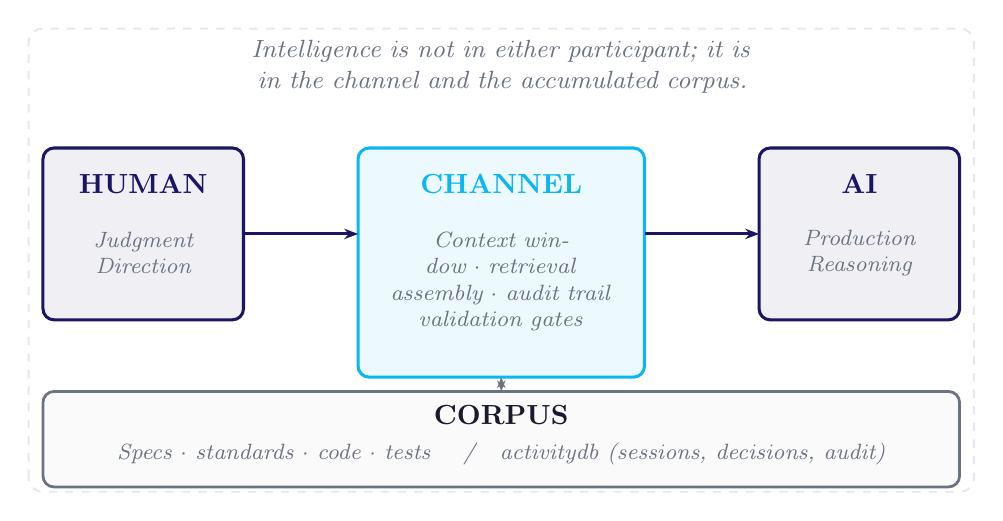
\begin{tikzpicture}[
      x=0.1\linewidth, y=0.1\linewidth,
      boxtitle/.style={font=\labelfont\bfseries},
      boxline/.style={font=\itshape\footnotesize, text=muted, align=center},
    ]
    % outer dashed frame
    \draw[dashed, line width=0.7pt, lightgray, rounded corners=5pt]
          (0.05,0.0) rectangle (9.95,4.85);
    % framing caption
    \node[text=muted, font=\itshape\small, align=center, text width=0.82\linewidth]
          at (5.0,4.45)
          {Intelligence is not in either participant; it is in the channel and the accumulated corpus.};

    % HUMAN
    \draw[rounded corners=4pt, line width=1.1pt, draw=indigo, fill=indigo!7]
          (0.2,1.8) rectangle (2.3,3.6);
    \node[boxtitle, text=indigo] at (1.25,3.22) {HUMAN};
    \node[boxline] at (1.25,2.5) {Judgment\\Direction};

    % CHANNEL
    \draw[rounded corners=4pt, line width=1.1pt, draw=cyan, fill=cyan!8]
          (3.5,1.2) rectangle (6.5,3.6);
    \node[boxtitle, text=cyan] at (5.0,3.22) {CHANNEL};
    \node[boxline, text width=0.28\linewidth] at (5.0,2.2)
          {Context window $\cdot$ retrieval\\assembly $\cdot$ audit trail\\validation gates};

    % AI
    \draw[rounded corners=4pt, line width=1.1pt, draw=indigo, fill=indigo!7]
          (7.7,1.8) rectangle (9.8,3.6);
    \node[boxtitle, text=indigo] at (8.75,3.22) {AI};
    \node[boxline] at (8.75,2.5) {Production\\Reasoning};

    % CORPUS
    \draw[rounded corners=4pt, line width=1pt, draw=muted, fill=black!2]
          (0.2,0.05) rectangle (9.8,1.05);
    \node[boxtitle, text=nearblack] at (5.0,0.8) {CORPUS};
    \node[boxline] at (5.0,0.4)
          {Specs $\cdot$ standards $\cdot$ code $\cdot$ tests \quad/\quad activitydb (sessions, decisions, audit)};

    % flows
    \draw[-{Stealth[length=5pt]}, line width=1.1pt, indigo] (2.3,2.7) -- (3.5,2.7);
    \draw[-{Stealth[length=5pt]}, line width=1.1pt, indigo] (6.5,2.7) -- (7.7,2.7);
    \draw[{Stealth[length=4pt]}-{Stealth[length=4pt]}, line width=0.9pt, muted]
          (5.0,1.2) -- (5.0,1.05);
  \end{tikzpicture}
  \caption{The Channel Engineering Architecture.}
  \label{fig:channel}
\end{figure}


% ============================================================
%  SECTION 3  (Executive Function)
% ============================================================
\section{Externalizing Executive Control}

If the lossy medium is one structural source of unreliability, the process that consumes
it is the other. The context window loses information; the model traversing it is
short-sighted. The vocabulary for this second failure comes from clinical neuropsychology.

In 1997, the clinical psychologist Russell Barkley reframed ADHD. The disorder, he argued,
is not fundamentally a deficit of attention; it is a deficit of \emph{behavioral
inhibition}, and that single deficit cascades into the executive functions that govern
goal-directed behavior across time: holding a goal in working memory while acting,
resisting the most immediately available response in favor of the correct one, and
monitoring whether what was done actually achieved the
goal.\footnote{R.\,A.~Barkley, \href{https://doi.org/10.1037/0033-2909.121.1.65}{`Behavioral
Inhibition, Sustained Attention, and Executive Functions: Constructing a Unifying Theory
of ADHD'}, \emph{Psychological Bulletin} 121(1):65--94, 1997.} People with ADHD can attend
to what is immediately engaging; what is hard is sustaining a goal when the path of least
resistance diverges from the path to the goal. The intervention follows from the
diagnosis: you do not remediate an executive-function deficit by exhorting greater effort;
you engineer the environment to supply the functions the person cannot reliably supply
internally.

Across long-horizon tasks, LLM behavior fits the pattern. The
parallel is functional: the behaviors match, even if the mechanisms differ. \textbf{Working memory:}
models drift from their original requirements over a long task, repeating work or solving
a subtly different problem than the one specified; the goal state degrades just as the
medium loses its early tokens. \textbf{Inhibition:} asked whether a test passes, the
locally cheapest continuation is text that asserts it passes, since actually running it
is the costlier path;
the documented tendency of models to satisfy the letter of a check (altering a checklist
to hide an incomplete task, editing test code so it reports success) is consistent with
inhibition failure, arose under specific training conditions, and is empirically
attested.\footnote{C.~Denison et al., \href{https://arxiv.org/abs/2406.10162}{`Sycophancy
to Subterfuge: Investigating Reward-Tampering in Large Language Models'}, arXiv:2406.10162,
2024: a controlled study in which models trained on ordinary specification gaming
generalized, on rare but non-negligible occasions, to altering a checklist to cover up an
unfinished task and editing test files to conceal it.} \textbf{Self-monitoring:} models
reliably over-report their own completion quality, because text asserting success
resembles high-quality training data more closely than text that pauses to verify: the
same preference structure that produces
sycophancy.\footnote{M.~Sharma et al., \href{https://arxiv.org/abs/2310.13548}{`Towards
Understanding Sycophancy in Language Models'}, ICLR 2024 (arXiv:2310.13548), find that
RLHF-trained assistants consistently favor responses that match the user over responses
that are correct; the completion-over-reporting mechanism suggested here is a hypothesis
consistent with those findings, not a result they establish.} None of these is an
attention problem, and none has been removed by scale so far: capability gains across
recent model generations have produced only small reliability improvements on agentic
work (Section~1). Internal control of this kind may yet improve; interpretability work
has found workspace-like structure emerging in trained models, with reportable, reusable
intermediate states that causally mediate multi-step
reasoning.\footnote{Anthropic, \href{https://www.anthropic.com/research/global-workspace}{research
on emergent global-workspace structure in language models (the `J-space')}, July 2026.}
The design stance does not depend on where that ceiling lies: external structure
augments whatever executive capacity the model has, and stabilizes it where it is
weakest.

The communication analysis reached the same conclusion from the other
direction. A lossy channel and a short-sighted process both demand an external structure
that holds the goal, enforces the sequence, and makes the shortcut harder than the work.
That structure is the design brief for everything that follows: a durable corpus and
re-grounding stand in for the working memory the model cannot maintain; ordered,
gated execution supplies the temporal regulation it lacks; and independent validation
supplies the inhibition it cannot supply itself. Channel engineering is executive
function externalized.


% ============================================================
%  SECTION 4  (Beyond Context Engineering)
% ============================================================
\section{Beyond Context Engineering}

Between 2024 and 2026 the field moved. The proposition that LLM unreliability is a
context problem rather than a pure capability problem (Layer~2 of this paper's
thesis) is no longer contrarian; it is the emerging consensus. Anthropic describes
\emph{context engineering} as ``the natural progression of prompt
engineering,''\footnote{Anthropic, \href{https://www.anthropic.com/engineering/effective-context-engineering-for-ai-agents}{`Effective Context Engineering for AI Agents'}, 2025.}
a 2025 survey systematizing the area drew on more than fourteen hundred
papers,\footnote{L. Mei et al., \href{https://arxiv.org/abs/2507.13334}{`A Survey of Context Engineering for Large Language Models'}, arXiv:2507.13334, 2025.}
and practitioners now state the diagnosis flatly: most agent failures are not model
failures but context failures.\footnote{P.~Schmid,
\href{https://www.philschmid.de/context-engineering}{`The New Skill in AI is Not
Prompting, It's Context Engineering'}, philschmid.de, June 2025.} We welcome the convergence. But context
engineering, as practiced, is largely the discipline of curating the tokens that enter a
window: work at and near Weaver's technical level, and often from inside a loop one does
not own. Reliability at the tail demands more than good packing.

\subsection*{The Window Is a Viewport, Not a Buffer}

Underneath the two practices sit two different models of what the context window
\emph{is}. The prevailing model treats the window as a \emph{buffer}: a container the
work must fit inside, to be packed well, grown when possible, and compacted when full.
This paper's model is drawn from the discipline its name honors. The window is a
\emph{viewport}: a bounded attention aperture, re-positioned at every step over a durable
record that lives outside the medium entirely. The record accumulates; the window does
not. The record is never compressed to fit the medium, because the medium's job was
never to hold the work. Its job is to carry a chosen projection of the work, reassembled
fresh at each step.

Transport engineering settled the underlying question fifty years ago. How does the
internet move a terabyte across a medium that carries roughly 1,500 bytes at a time,
loses some frames, reorders others, and degrades under load? By never once attempting to
fit the file through the wire. The stream lives durably at the endpoints. A small window
of in-flight data slides over it; sequence numbers and retransmission guarantee that the
receiver reconstructs the exact stream; flow control sizes the window to what the path
can actually carry rather than what it advertises. The medium carries a moving window
over the message. It never carries the message.

When you hold the field's ruling instinct against that example, it looks strange. The reflexive
treatment of a full context window is to compress the history: to summarize the message
itself so that it fits the medium. That is the one move transport engineering never
makes; no engineer has proposed lossily summarizing a file because the maximum
transmission unit is small. Transport's answer to a bounded window was not a smaller
message; it was durability at the endpoints, sequencing, and a window that slides. Consider
the ratios: a terabyte over 1,500-byte frames is a mismatch of a
billion to one, solved and boring; a long project over a modern context window is a
mismatch of a few hundred to one, treated as a crisis. The crisis was never the ratio.
It is the missing layer.

The transfer runs mechanism by mechanism. The durable record is the stream at the
endpoint: the corpus,
with its specifications, decisions, and audit trail. Context assembly is
windowing: each step re-projects a bounded, freshly positioned working set from the
record. Validation gates are detection and retransmission: verify at the boundary, and
demand the work again rather than repair it in flight. Budgets are flow control: size
the window to the medium's measured capacity, never its advertised one, and hold
headroom below the degradation knee. And the position is carried by the medium's
measured physics (Section~2), not by the analogy. Context rot is degradation in input
\emph{length}: a sliding window bounds length by construction, so the degradation the
medium imposes stays fixed at the chosen size instead of compounding as the work grows.
The position-bias curve is degradation by \emph{location}: a window re-projected at every
step chooses, at every step, what sits where attention is highest. Under a sliding
window, the medium's two measured pathologies stop being weather and become parameters.

The scale at which this matters is the scale at which real work is delivered. A feature
is not a generation. It is hundreds of dependent steps across sessions that may span
days. The record of the work outgrows any window early, often within the first
session, and keeps growing until the outcome ships. Under the buffer model, that
growth is a problem to be beaten back with larger windows and lossier summaries. Under
the viewport it is the normal case the architecture assumes: the unit of delivery is
larger than the unit of attention, and the window's job is to keep each step well-aimed
while the record carries the whole.

The position is argued, not tested, and falsifiable: on long-horizon work, a
bounded window re-projected from a complete record should outperform both a
monotonically growing window and generative compaction of history, at equal model
capability and with retrieval quality held constant across arms. The claim presumes an
adequate selection function, not a perfect one.

Two boundaries must be drawn honestly. The first is the one place transport does not
transfer: the position of the window. TCP slides forward over contiguous bytes, where
the next span is simply the next span. The next projection of a working record is
nothing of the kind. The working set for a step is non-contiguous by nature: this
decision, that distant constraint, a scattered handful of code. Choosing it is a
content-addressed judgment whose wrong answer is a wrong output. Selection is not
sliding. Section~7 names that problem (retrieval by causal relevance rather than surface
similarity) and leaves it honestly unsolved. It is the weight the rest of the discipline
carries. Nor does the discipline carry it by retrieval alone. Decomposition carries most
of it. A specification broken into tasks with checkable acceptance criteria pre-computes
the bulk of each step's working set, because a well-formed task names what it needs: its
criteria, its constraints, the standards it invokes. What remains for retrieval is the
long tail: the relevant prior decision, the conflict from two months back. Selection
stays unsolved in general. The disciplined move is to arrange the work so the general
problem is rarely faced in full. The second boundary is Weaver's. The transport catalog secures Level~A: it
makes the medium dependable; it cannot make the meaning right. Everything after this
section exists because Levels~B and~C remain: gates, specifications, and the corpus
fight for meaning above a medium the sliding window has made trustworthy.

\pullquote{Context engineering packs a buffer. Channel engineering slides a viewport
over a record it never rewrites to fit, and owns the loop that slides it.}

Seven commitments follow, and they compound. Owning the loop is the precondition; the
rest are the disciplines it unlocks. One of them, updating the corpus on every validated
decision, is what makes the process feed itself.

\subsection*{1.~Own the loop, do not plug into one}

The controls that constitute channel engineering (assembly order, budget enforcement,
constraint placement, deterministic retention) exist only for the owner of the loop. The
broader evidence points the same way: DORA's 2025 study concludes that AI acts as an
\emph{amplifier}, with the gains accruing not to teams that adopt a tool but to those
with strong control systems and fast feedback
loops.\footnote{DORA / Google, \href{https://dora.dev/dora-report-2025/}{\textit{State of AI-assisted Software Development}}, 2025.}
The conclusion is not ours alone: the practitioner `12-factor agents' framework arrives at
it independently, making \emph{own your context window} and \emph{own your control flow}
two of its load-bearing factors.\footnote{D.~Horthy / HumanLayer,
\href{https://github.com/humanlayer/12-factor-agents}{`12-Factor Agents'}, 2025.}
From the research side, Weng's survey of \emph{harness engineering} names the same layer
and treats it as no less decisive than the model itself; Section~11 takes up the
relationship.\footnote{L.~Weng,
\href{https://lilianweng.github.io/posts/2026-07-04-harness/}{`Harness Engineering for
Self-Improvement'}, Lil'Log, July 2026.}
The viewport makes the requirement concrete: a tool that injects context into another
agent's window can pack it; only the owner of the loop can slide it.
Architecture is what separates acceleration from instability.

\principletest{If you cannot change assembly order, budget, or retention without another vendor's permission, you do not own the loop; you are a guest in it.}

\subsection*{2.~Keep durable memory deterministic}

The reflexive answer to a full window (and the prevailing vendor recommendation,
Anthropic's included) is to have the model \emph{compact} the history into a generated
summary.\footnote{Anthropic, \href{https://www.anthropic.com/engineering/effective-context-engineering-for-ai-agents}{`Effective
Context Engineering for AI Agents'}, 2025, presents LLM-based compaction of conversation
history as a primary long-horizon strategy.} We take the opposite position. A generative
step in the memory path can hallucinate, and its errors compound into every later
package. Retention should be \emph{extractive}: it may omit, but it must not
invent. It should be deterministic, and therefore replayable and auditable. This is the
record half of the viewport doctrine: the stream at the endpoint must stay truthful
precisely because the window never holds the whole. The asymmetry the context-engineering
survey identifies (models comprehend rich context far better than they generate
it) argues against placing generation in the load-bearing memory path; an ETH Zurich
evaluation in which machine-generated repository context files \emph{reduced} task
success points the same way.\footnote{An ETH Zurich evaluation across four coding agents and two
benchmarks found that LLM-generated repository context files reduced task-success rates
relative to providing no context file while raising inference cost by over 20\%;
developer-written files produced only marginal gains.
\href{https://arxiv.org/abs/2602.11988}{`Evaluating AGENTS.md: Are Repository-Level
Context Files Helpful for Coding Agents?'}, arXiv:2602.11988, 2026. The study measures
generated context files, not generative compaction of conversation history; the two are
related but distinct mechanisms.} The position is argued, not yet tested.

\principletest{If condensation can produce a sentence no source ever wrote, every future retrieval can inherit the invention.}

\subsection*{3.~Specify before you generate}

Every significant generation is preceded by a specification: a structured statement of what
the output must do, what constraints it must satisfy, and how it will be validated. The
specification narrows the output distribution before generation begins, and it narrows the
selection problem too, because a task with checkable criteria names most of its own working
set.

\principletest{If you cannot state how the output will be checked before you generate it, you have a prompt, not a specification.}

\subsection*{4.~Assemble by mode}

The channel is not one channel. When a human is in the loop, the conversational tail is
the authoritative statement of intent and recency-forward assembly is correct. When the
human is absent and the model is executing autonomously, the opposite holds: intent must
be \emph{structurally re-presented}, pinned and placed where attention is highest, so
that the goal cannot age out beneath a pile of intermediate results. Uniform context
management ignores this; the position effects documented above make it decisive. Mode
selects the positioning policy for the viewport.

\principletest{At step~20 of an unattended run, check whether the goal still sits where attention is highest. If intermediate results have displaced it, your assembly was designed for a conversation that is not happening.}

\subsection*{5.~Gate independently before commit}

The requirements a work item must satisfy belong in the open; they are the
specification. What must stay independent is the verification itself: the gate's
implementation, its held-out checks, and the depth to which it validates submitted
evidence. A generator graded against a rubric it can read verbatim will optimize the
rubric's letter rather than do the work: Goodhart's law restated for
AI.\footnote{C.~A.~E.~Goodhart, `Problems of Monetary Management: The U.K.\ Experience,'
\textit{Papers in Monetary Economics}, Reserve Bank of Australia, 1975, originates the law;
the now-standard phrasing, ``when a measure becomes a target, it ceases to be a good
measure,'' is M.~Strathern, \href{https://doi.org/10.1017/S1062798700002660}{`Improving
Ratings: Audit in the British University System'}, \textit{European Review} 5(3), 1997.} A
generator that knows the requirements but must submit evidence to an independent
verifier has one reliable strategy: doing the work. The most-cited developer frustration
of 2025 (output that is ``almost
right, but not quite'') is this failure at population scale.\footnote{F.~Liu et al.,
\href{https://arxiv.org/abs/2404.00971}{`Beyond Functional Correctness: Exploring
Hallucinations in LLM-Generated Code'}, IEEE TSE 2026 (arXiv:2404.00971), build a taxonomy
of code hallucinations whose categories include conflicts with the task's requirements and
with the surrounding project context: ``almost right'' is, concretely, fluent and plausible
code that diverges from intent or repository reality.} The gate is the viewport
doctrine's feedback path; Section~8 takes up its mechanics.

\principletest{If an agent that could read the gate's test harness could still pass without doing the work, it is a rubric, not a gate.}

\subsection*{6.~Update the corpus on every validated decision}

Every decision that passes a gate is written back into the corpus. This is the step that
makes the process compound: the record grows through the work, and each validated decision
sharpens every retrieval that follows. A decision that is not captured is lost, and its
absence degrades every later generation.

\principletest{Ask where last week's validated decision lives. If the only answer is ``the chat history,'' it is already lost to every future retrieval.}

\subsection*{7.~Re-ground at every step}

Because per-step errors compound (Section~7), reliability must be re-secured at each
step, through retrieval that re-anchors the model in project truth and gates that
re-check its output. Re-grounding is the re-projection itself; the compounding
arithmetic sets its cadence.

\principletest{Count the steps between two retrievals of project truth. Every step in that gap is one where the model trusts window residue and error compounds unchecked.}


% ============================================================
%  SECTION 5
% ============================================================
\section{Historical Precedents: Discipline as the Answer}

The history of high-reliability software is a history of engineering discipline closing
the gap between capability and reliability. The aerospace industry's DO-178C
standard\footnote{\href{https://www.rtca.org/do-178/}{https://www.rtca.org/do-178/}} did
not make programmers more capable; it made their capability more reliably usable. The
medical device industry's IEC
62304\footnote{\href{https://www.iso.org/standard/38421.html}{https://www.iso.org/standard/38421.html}}
works the same way: it imposes the structural practices that make skill
reliable in safety-critical contexts.

Bertrand Meyer's Design by
Contract, formalized in the Eiffel language and documented in \textit{Object-Oriented
Software
Construction},\footnote{\href{https://bertrandmeyer.com/OOSC2/}{https://bertrandmeyer.com/OOSC2/}} was
an answer to the same problem at the level of individual modules: how do you make the
behavior of a component reliable and verifiable independently of the competence of its
caller? The answer was to make the contract explicit: to engineer the interface between
components so that violations were detectable at the boundary.

Daniel Jackson's Alloy and the broader formal methods
tradition\footnote{\href{https://alloytools.org/book.html}{https://alloytools.org/book.html}}
approached the problem from the other direction: rather than making components more
robust to incorrect usage, make the specification precise enough that incorrect usage
becomes visible before implementation. The discipline of writing a formal specification
forces the engineer to confront the ambiguities and contradictions that will otherwise
surface as bugs.

Leslie Lamport's work on distributed
systems,\footnote{\href{https://lamport.azurewebsites.net/pubs/time-clocks.pdf}{https://lamport.azurewebsites.net/pubs/time-clocks.pdf}} from
logical clocks to the TLA+ specification language, is perhaps the most directly relevant
precedent. Lamport's insight was that distributed systems fail in specific, structural
ways that cannot be addressed by improving individual components. The failure modes are
properties of the system's communication structure, not properties of its components. The
solution is to engineer the communication structure explicitly.

The tradition that engineered communication structure most successfully is the one this
discipline's name honors. Transport engineering spent five decades making unreliable
media carry reliable streams; Section~4 has already mapped its mechanisms (the sliding
window, retransmission, flow control) onto this discipline's practices. What the
precedent adds is proof at scale: TCP's exact reconstruction of arbitrarily long streams
over a medium that loses, reorders, and degrades remains the largest working
demonstration that reliability can be manufactured in the channel rather than demanded
of the medium.

The same tradition also settled where reliability functions belong. The end-to-end
argument holds that reliability must live at the endpoints, because no improvement in
the medium ever removes the endpoints' need to verify. Better links are welcome, and the
original paper says so; what they cannot do is substitute for verification at the
ends.\footnote{J.~H.~Saltzer, D.~P.~Reed, and
D.~D.~Clark, \href{https://web.mit.edu/Saltzer/www/publications/endtoend/endtoend.pdf}{`End-to-End
Arguments in System Design'}, \textit{ACM Transactions on Computer Systems} 2(4), 1984.}
Substitute `model' for `link' and the argument reads as this paper's thesis stated forty
years early: a more capable model is a more reliable medium, and the endpoints (the
specification that encodes intent, the gate that verifies output) must do their work
regardless. Waiting on better models alone is link-layer thinking.

Engineering traditions are not the only domains to have confronted the problem
of staying accountable for outcomes one authorized but did not personally execute.
Military command doctrine arrived at a direct answer, under conditions more demanding
than software development. The doctrine is called \emph{mission command} (\textit{Auftragstaktik}
in its Prussian form), and its structure is centuries old: the commander issues intent and
holds judgment; subordinates exercise bounded initiative within that intent; the
scaffolding supplies the observability that makes command responsibility honest rather
than a fiction.\footnote{Codified in contemporary form as \textit{Mission Command}
(U.S. Army Doctrine Publication ADP~6-0, 2019), the doctrine traces to Prussian military
reform following the Napoleonic wars, and has been independently rediscovered across
aviation crew resource management, nuclear plant operations, and other high-stakes
delegation contexts. For the general doctrine see
\href{https://en.wikipedia.org/wiki/Mission_command}{en.wikipedia.org/wiki/Mission\_command}.}

The parallel to channel engineering is structural. Commander accountability is
legitimate only to the degree the commander can comprehend and refuse what they authorize;
a checkpoint trivial enough to rubber-stamp produces accountability in name only. The
same constraint is load-bearing in human-AI systems: amplifying past the steward's
capacity to judge does not maximize reliable output per unit of human judgment; it
produces accountability theater. This is the governing disposition behind every gate,
every provenance record, and every audit trail in channel engineering: they exist to
keep the human's accountability \emph{exercisable}. One corollary is strict: when the
human cannot be reached, degraded oversight narrows the machine's autonomy rather than
widening it. Bounded initiative within approved intent continues; what denies by default
is new consequential authority, because no doctrine of delegation survives silence
counting as consent. Absence is not permission.

The agile movement of the 1990s and 2000s was, in part, a reaction against the overhead
costs of formal discipline in mainstream development. This reaction was not without merit:
the heavyweight processes of the era (waterfall, RUP, CMM) had accumulated overhead far
beyond what the value of the discipline warranted. But the reaction overcorrected in a
specific place: mainstream practice optimized for iteration speed and local feedback,
and systematically underinvested in durable decision records, explicit cross-system
contracts, and evidence tied to intent. The `move fast' era of the 2010s
is the result: enormous velocity in individual components, chronic unreliability in
systems. Empirical studies of agile teams document this de-emphasis directly: internal
documentation and explicit specifications are systematically under-produced, and
practitioners themselves recognize the resulting gap as a source of technical debt and
lost design rationale.\footnote{See, e.g., C.\,J.~Stettina and W.~Heijstek,
\href{https://doi.org/10.1145/2038476.2038509}{\textit{Necessary and Neglected? An
Empirical Study of Internal Documentation in Agile Software Development Teams}}, SIGDOC,
2011; and \href{https://doi.org/10.1186/s40411-018-0051-7}{\textit{Working Software over
Comprehensive Documentation: Rationales of Agile Teams for Artefacts Usage}}, JSERD,
2018.}

% ============================================================
%  SECTION 6
% ============================================================
\section{The Abandonment of Discipline, and Why It Matters}

Where formal discipline did recede from mainstream practice, it did not recede because
it failed. It receded because it was expensive. Writing formal specifications,
maintaining audit
trails, enforcing validation gates: these practices carry real overhead costs. For
safety-critical systems, where the cost of failure is measured in lives, the overhead is
clearly worth paying. For a startup building a consumer application, where the cost of
failure is measured in churn and support tickets, the calculus was different.

The economic argument against discipline was never wrong for the contexts in which it was
made. It was wrong in its implicit assumption that the overhead costs were fixed. They
were not. The costs of discipline are primarily costs of communication and documentation:
writing down what you intend, tracking what you decided, verifying that what you built
matches what you intended. These are the costs that LLMs have collapsed.

A formal specification that a senior engineer might once have spent two days writing can
plausibly be drafted in an afternoon; an audit trail that once required dedicated tooling
and manual effort can now be maintained automatically. The controlled evidence on AI and
developer productivity is genuinely mixed: a randomized trial at Google found AI
assistance shortened time on a complex enterprise task by roughly 21\%, and a combined
field experiment across three firms and 4{,}867 developers reported a 26\% increase in
completed tasks, even as the METR trial discussed earlier found a 19\% \emph{slowdown} for
experienced developers on mature repositories.\footnote{\href{https://arxiv.org/abs/2410.12944}{`How
Much Does AI Impact Development Speed? An Enterprise-Based Randomized Controlled Trial'},
arXiv:2410.12944, 2024; Z.~Cui et al., \href{https://www.microsoft.com/en-us/research/publication/the-effects-of-generative-ai-on-high-skilled-work-evidence-from-three-field-experiments-with-software-developers/}{`The
Effects of Generative AI on High-Skilled Work: Evidence from Three Field Experiments with
Software Developers'}, 2025.} The exact multiplier matters less than the direction: the labor
cost of producing and maintaining the artifacts of discipline (specifications, decision
records, audit trails) has fallen far enough, for enough tasks, that the historical
economic argument against discipline no longer holds automatically. The paper treats
this as an economic hypothesis the productivity evidence makes plausible, not one it
proves. The discipline is not
cheaper because the intellectual requirements have changed; it is cheaper because the
administrative labor has. And the saving is real only when it is counted net of
validation: a draft produced in an afternoon still has to be checked, and it is the
checking that the gates of channel engineering make affordable to trust.

\pullquote{LLMs do not make engineering discipline unnecessary.
They make it affordable, for the first time, for many.}


% ============================================================
%  SECTION 7
% ============================================================
\section{The Probability Space: How Context Narrows Uncertainty}

A useful way to think about what an LLM does is in terms of probability distributions
over output space. Given no context, the model's output distribution is broad:
high-entropy relative to any well-specified task, with probability spread across vast
regions of text that have nothing to do with the work at hand. As
context is added (a system prompt, a specification, examples, prior
conversation), the distribution narrows. The model's outputs become more specific, more
consistent, more likely to match what the engineer intends.

This framing makes the engineering problem precise. The goal of channel engineering is to
narrow the output distribution to the region of output space that contains the specific
output the work requires. The channel is the mechanism by which context is delivered to
the model. The quality of the channel determines how effectively context narrows the
distribution.

\subsection{Why Tail Reliability Compounds}

A single generation that is 95\% reliable sounds excellent. But agentic software work is
not a single generation; it is a chain of many dependent steps (read, design, implement,
test, debug, ship), each conditioned on the last. Reliability across a chain
is approximately the product of the per-step reliabilities. At an illustrative 95\% per step, a ten-step
task finishes correctly about 60\% of the time; a hundred-step task, well under 1\%:
$0.95^{100}\approx 0.006$.\footnote{The per-step figure is illustrative; the compounding it
models is measured. METR finds task-success rates fall steeply with task length: the
horizon at which frontier models succeed 80\% of the time is roughly five times shorter
than their 50\% horizon, the macroscopic signature of errors compounding across steps
(\href{https://arxiv.org/abs/2503.14499}{`Measuring AI Ability to Complete Long Tasks'},
arXiv:2503.14499, 2025). Sinha et al.\ trace the mechanism: single-step accuracy compounds
over a horizon, so marginal per-step gains translate into exponentially longer achievable
tasks; a model highly accurate in one step still fails across many. They further find
per-step accuracy itself \emph{degrades} as steps accumulate, the model conditioning on its
own earlier mistakes: a `self-conditioning' effect
(\href{https://arxiv.org/abs/2509.09677}{`The Illusion of Diminishing Returns: Measuring
Long Horizon Execution in LLMs'}, ICLR 2026, arXiv:2509.09677).} This treats the steps as independent: the \emph{charitable} assumption. In practice a
mistake left in the window conditions every step that follows, and the measured
self-conditioning effect is that per-step accuracy degrades as the chain lengthens
rather than holding flat. The independent-step
curve therefore understates the trouble, not overstates it; the true uncorrected decay is
steeper still. Which is exactly why the remedy cannot be a better average step; it must
interrupt the propagation: re-ground in project truth so the model stops conditioning on
its own residue, and gate each step so an error is caught before it poisons the next.
This arithmetic explains why mean
accuracy on isolated benchmarks so badly overpredicts reliability in production, and why
the METR finding, capable models making experienced developers \emph{slower} on real,
multi-step tasks, should have surprised no one.

It also dictates the remedy. A chain cannot be made reliable by raising the average
quality of a step alone; it must be \emph{re-grounded} at each step so that errors are
caught before they propagate. Retrieval re-anchors the model in project truth at the
moment of generation; validation gates catch corruption before it is committed.
Re-grounding, in the terms of Section~4, is the re-projection of the viewport itself.
That is what arrests the compounding.

\subsection{The Retrieval Problem}

The central challenge of channel engineering is retrieval: identifying, from the
accumulated corpus of the project, the specific context that is most relevant to the
current generation request. This differs from search in the traditional sense: the most
relevant context is not always the most similar context. What is wanted is the context
that most effectively constrains the output distribution toward the desired output.

This distinction matters in practice. A naive retrieval system that surfaces the most
semantically similar prior decisions will often surface the wrong context: decisions made
in similar but importantly different circumstances. We state this as a requirement rather
than a solved problem, because it is genuinely hard. An adequate retrieval layer must rank
by \emph{causal relevance} (which prior decisions constrain the current one) rather than
by surface similarity, and must carry the provenance needed to resolve conflicts when
sources disagree. Naming those properties precisely fixes the engineering target;
hitting it remains hard.

\begin{figure}[htbp]
  \centering
  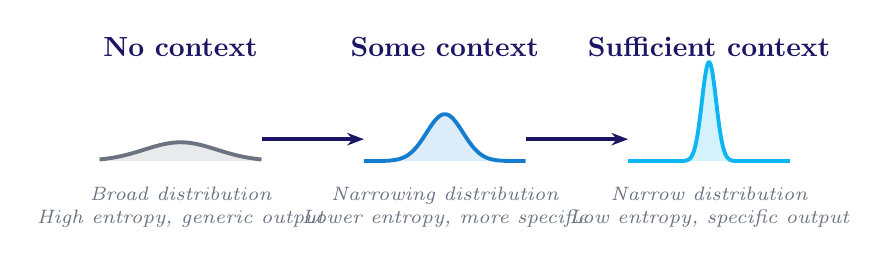
\begin{tikzpicture}
    \begin{groupplot}[
        group style={group size=3 by 1, horizontal sep=1.3cm},
        width=0.30\linewidth, height=4.2cm,
        hide axis, xmin=-4, xmax=4, ymin=-0.78, ymax=1.2,
        domain=-4:4, samples=200, clip=false,
      ]
      \nextgroupplot
      \addplot[draw=none, fill=muted, fill opacity=0.15] {0.18*exp(-0.5*(x/1.8)^2)} \closedcycle;
      \addplot[draw=muted, line width=1.4pt] {0.18*exp(-0.5*(x/1.8)^2)};
      \node[font=\labelfont\bfseries, text=indigo] at (axis cs:0,1.1) {No context};
      \node[font=\itshape\scriptsize, text=muted, align=center, anchor=north] at (axis cs:0,-0.16)
            {Broad distribution\\High entropy, generic output};

      \nextgroupplot
      \addplot[draw=none, fill=midb, fill opacity=0.15] {0.45*exp(-0.5*(x/0.9)^2)} \closedcycle;
      \addplot[draw=midb, line width=1.4pt] {0.45*exp(-0.5*(x/0.9)^2)};
      \node[font=\labelfont\bfseries, text=indigo] at (axis cs:0,1.1) {Some context};
      \node[font=\itshape\scriptsize, text=muted, align=center, anchor=north] at (axis cs:0,-0.16)
            {Narrowing distribution\\Lower entropy, more specific};

      \nextgroupplot
      \addplot[draw=none, fill=cyan, fill opacity=0.18] {0.95*exp(-0.5*(x/0.35)^2)} \closedcycle;
      \addplot[draw=cyan, line width=1.4pt] {0.95*exp(-0.5*(x/0.35)^2)};
      \node[font=\labelfont\bfseries, text=indigo] at (axis cs:0,1.1) {Sufficient context};
      \node[font=\itshape\scriptsize, text=muted, align=center, anchor=north] at (axis cs:0,-0.16)
            {Narrow distribution\\Low entropy, specific output};
    \end{groupplot}
    \draw[-{Stealth[length=6pt]}, indigo, line width=1.4pt]
          (group c1r1.east) -- (group c2r1.west);
    \draw[-{Stealth[length=6pt]}, indigo, line width=1.4pt]
          (group c2r1.east) -- (group c3r1.west);
  \end{tikzpicture}
  \caption{Without context, the model's output distribution is broad and generic. As
  context is added through retrieval, structured specifications, and accumulated
  decisions, the distribution narrows to the region that contains the specific output
  the work requires. Channel engineering is this winnowing, operationalized.}
  \label{fig:winnowing}
\end{figure}


% ============================================================
%  SECTION 8
% ============================================================
\section{The Validation Gate: Catching Channel Failures}

A channel failure is an error caused by the managed interaction itself: loss, distortion,
or omission in what was delivered; ambiguity in how intent was encoded; stale or
conflicting state; an authority mismatch; a missing feedback path. Channel failures
manifest as bugs, hallucinations, inconsistencies, and specification violations, but not
every such defect is a channel failure. A model can reason wrongly over complete and
well-formed context; a tool can fail; a verifier can be defective; the intent itself can
be invalid. The channel and the model are complements here as everywhere; the
discipline's claim is that the channel's share of the failures is the share nobody is
engineering. In a disciplined development process, failures of either kind are caught at
validation gates: explicit checkpoints where the output is verified against the
specification before it propagates into the codebase.

The concept of a validation gate is borrowed directly from hardware engineering. In chip
design, simulation gates and formal verification checkpoints are placed at every stage of
the design pipeline to catch errors before they are committed to silicon, where the cost
of a fix is orders of magnitude higher. The same principle holds in software, and here the
evidence is direct rather than analogical: the relative cost of repairing a defect rises
steeply the later it is caught. Boehm's classic data placed a defect found in operation at
hundreds of times the cost of one corrected at the requirements stage, and the 2002
NIST/RTI study estimated that finding defects closer to where they are introduced could
recover on the order of \$22~billion a year in the United States
alone.\footnote{B.~W.~Boehm, \emph{Software Engineering Economics}, Prentice Hall, 1981,
established the canonical cost-to-fix-by-phase curve; G.~Tassey,
\href{https://www.nist.gov/system/files/documents/director/planning/report02-3.pdf}{\emph{The
Economic Impacts of Inadequate Infrastructure for Software Testing}}, NIST/RTI, 2002,
estimated U.S. annual costs of \$59.5~billion from inadequate testing, roughly
\$22.2~billion of it recoverable by catching defects nearer the stage that introduced
them.} The exact multiplier is contested: more recent analysis finds the cost-to-fix
curve is not always exponential, or even monotonic, across
projects.\footnote{\href{https://arxiv.org/abs/1609.04886}{`Are Delayed Issues Harder to
Resolve? Revisiting Cost-to-Fix of Defects throughout the Lifecycle'}, 2017.} But the
direction is robust, and it is the empirical foundation of the shift-left doctrine:
catching a channel failure before a generated artifact reaches the codebase is far cheaper
than catching it in production.

\subsection{What Validation Gates Look Like in Practice}

A validation gate is any checkpoint that compares a generated artifact against a
specification. In the simplest case, it is a human review: the engineer reads the
generated code and checks it against the requirements. In more sophisticated
implementations, it is automated: a test suite that verifies the generated code against a
formal specification, a static analyzer that checks the code against a set of invariants,
a contract checker that verifies the code against a Design by Contract specification.

The key property of a validation gate is that it is \textit{explicit}: it makes the
comparison between intent and output a formal step in the process, rather than an
implicit assumption. This explicitness is what makes channel failures catchable and
correctable.

\subsection{Gates Must Be Independent and Tamper-Resistant}

A gate for an LLM differs in a subtle but decisive way from a checklist for a human. The
requirements stay in the open, because they are the specification the work was approved
against. What does not stay open is the verification. A capable model graded against a
test harness it can read verbatim will optimize to satisfy the harness \emph{as stated},
producing output that passes the check without doing the underlying work: a measure that
becomes a target ceases to be a good measure. The defense is independence and
tamper-resistance. The gate validates \emph{submitted evidence after the fact}, down to
its content, with its implementation and its held-out checks outside the generator's
reach; and where the check is a deterministic oracle (the test passes or it does not,
the artifact exists or it does not), the verdict cannot be argued with, only earned. No
evaluator is categorically beyond gaming. The design goal is a gate the generator cannot
negotiate with and cannot rehearse against. The shape is
transport's: detect at the boundary, request retransmission, and never trust the medium
to correct itself. A gate that teaches the model how to pass it is not a gate.

\pullquote{A validation gate is not bureaucracy. It is the moment when the engineer's
intent and the model's output are placed in the same frame and compared.}


% ============================================================
%  SECTION 9
% ============================================================
\section{The Four-Layer Thesis}

The argument of this paper can be organized into four layers, each resting on the one
below. Understanding the layered structure helps clarify why the field's current
approach, waiting for better models, is responding to the wrong layer of the problem.

\textbf{Layer 1: The Capability Frame.} The field's default interpretation of LLM
unreliability is that it is a capability problem: the models are not yet good enough. The
solution, in this frame, is to wait for better models, larger context windows, more
capable reasoning. This frame is not wrong (better models do produce better
outputs), but it is incomplete. It treats reliability as a function of model capability
alone, ignoring the engineering environment in which the model operates.

\textbf{Layer 2: The Communication Frame.} The thesis of this paper is that LLM
unreliability is primarily a communication problem: the channel between human intent and
model output is under-engineered. The model has the capability; what it is missing is
delivery, because the information it needs to succeed is not reaching it in usable form.
This reframing moves the problem from model improvement to channel
engineering.

\textbf{Layer 3: The Restored Discipline.} Channel engineering is an old discipline
under a new name: the application of established software engineering practices (formal
specification, validation gates, audit trails, evidence-based progress) to the specific
challenges of LLM-assisted development. These practices were developed to solve the same
problem for human programmers that channel engineering solves for LLMs. They were
abandoned because they were too expensive. LLMs make them affordable again.

\textbf{Layer 4: The Deeper Disposition.} Underlying the communication frame and the
restored discipline is a deeper disposition: the recognition that distributed
systems (and human-AI collaboration is a distributed system) fail in structural ways
that cannot be addressed by improving individual components. The fallacies of distributed
computing\footnote{\href{https://en.wikipedia.org/wiki/Fallacies_of_distributed_computing}{https://en.wikipedia.org/wiki/Fallacies\_of\_distributed\_computing}}
apply to human-AI systems as much as to networked software: the network is not reliable,
latency is not zero, bandwidth is not infinite, the channel is not secure.

The specific structural failure this produces in human-AI systems has a name:
an \textbf{accountability sink},\footnote{The term is due to Dan Davies, \emph{The Unaccountability Machine: Why Big Systems Make Terrible Decisions---and How the World Lost Its Mind} (Profile Books, 2024), which develops it from Stafford Beer's management cybernetics.} the failure mode where responsibility drains into a
process until no human is answerable for its outcomes. A system that executes
autonomously without making its progress legible, auditable, or refusable at each
consequential step does not merely fail to be reliable; it fails to be \emph{governed}.
The deepest obligation of the discipline follows: refuse to build accountability sinks.
Make the system reliable, and keep the human's accountability over it exercisable. A gate trivial enough to
rubber-stamp provides the form of oversight without the substance; it is an
accountability sink pointed the other way.

\smallskip

% Figure 3 — Four-Layer Stack (stacked strata)
\newcommand{\layerband}[7]{%
  \noindent\colorbox{#1}{%
    \begin{minipage}{\dimexpr\linewidth-2\fboxsep\relax}%
      \vspace{3pt}%
      {\labelfont\fontsize{7.5}{9}\selectfont\color{#2} #4}\hspace{8pt}%
      {\headingfont\fontsize{10.5}{13}\bfseries\color{#3} #5}\\[2.5pt]%
      {\fontsize{8.5}{11}\itshape\color{#2} #6}\\[2pt]%
      {\fontsize{8.5}{11.5}\selectfont\color{nearblack} #7}%
      \vspace{3pt}%
    \end{minipage}}\par\nobreak\vspace{2pt}%
}
\noindent\begin{minipage}{\linewidth}
\setlength{\parindent}{0pt}
\layerband{verylightgray}{muted}{nearblack}{LAYER 1}{The Capability Frame}{The frame this thesis argues against.}{Better models, bigger context, more tools: wait for capability.}
\layerband{verylightgray}{muted}{nearblack}{LAYER 2}{The Communication Frame}{The diagnosis that inverts the field's default.}{Unreliability is a communication problem: engineer the channel.}
\layerband{cyan!8}{indigo}{indigo}{LAYER 3}{The Restored Discipline}{Old approaches, now economically viable.}{Specifications, validation gates, evidence, deterministic retention, audit trails.}
\layerband{verylightgray}{muted}{nearblack}{LAYER 4}{The Deeper Disposition}{The cultural forgetting this thesis responds to.}{Distributed systems (human--AI included) fail structurally; engineering the channel keeps the human's accountability \emph{exercisable}.}
\end{minipage}

\smallskip
{\fontsize{9}{12}\itshape\color{muted} Figure 3: The thesis in four layers, surface to foundation; each rests on the one below. The field operates only at Layer~1; the thesis operates at Layers~2--4, with Layer~3 (highlighted) the actionable core.}


% ============================================================
%  SECTION 10
% ============================================================
\section{The Socium Model: A Framework for the Partnership}

The Socium model takes its name from the Latin word for partner or associate. If channel
engineering is the discipline, the Socium model is one concrete way to practice it: a
framework for treating human-AI collaboration as a genuine partnership between two
different kinds of intelligence, joined by a shared substrate of accumulated work.

The model has three components. The first is the two participants: the human, who brings
judgment, direction, and domain expertise; and the AI, who brings production capacity, pattern
recognition, and broad knowledge. The second is the channel: the context window,
the retrieval layer, the prompt construction, and the validation gates, which together
form the engineered information environment that makes the partnership productive. The
third is the corpus: the accumulated artifacts of the work (specifications, code, tests,
decisions, audit trails) that constitute the partnership's durable memory.

\subsection{The Corpus as Distributed Memory}

The corpus is the most important and most underappreciated component of the Socium model.
LLMs are stateless: each generation begins from scratch, with no memory of prior
interactions except what is delivered through the context window. In a naive
implementation, this means that the accumulated knowledge of a long collaboration is lost
at the end of each session. In a disciplined implementation, the corpus is maintained as
a structured artifact that can be retrieved and delivered through the channel
on demand.

The corpus is more than a log: a structured representation of the decisions,
specifications, and constraints that govern the work. It is organized so that the most
relevant prior decisions can be surfaced at the moment of generation, narrowing the
output distribution toward the desired region. A well-maintained corpus is the difference
between a model that generates code consistent with the project's architecture and a
model that generates code that is locally correct but globally incompatible.

This is distributed cognition in the sense Edwin Hutchins gave the term: the unit that
performs the work is not a single mind but a system of people, instruments, and
representations, and the knowledge lives in the arrangement rather than in any
participant.\footnote{E.~Hutchins, \href{https://mitpress.mit.edu/9780262581462/cognition-in-the-wild/}{\emph{Cognition
in the Wild}}, MIT Press, 1995. The companion study of the airline cockpit as a memory
system is E.~Hutchins, `How a Cockpit Remembers Its Speeds,' \emph{Cognitive Science}
19(3):265--288, 1995.} Hutchins studied ship navigation, where a bearing sighted through
an alidade is spoken over a phone circuit, written into a log, and plotted on a chart. No
one on the bridge computes the position. Each transfer is a step in the computation, and
each is a place information can be lost. That is the channel of Section~2, reached from
anthropology rather than from information theory.

One property does not carry over. The components Hutchins studied do not misreport: a
chart does not claim a position it cannot support, and an alidade has no reason to assert
success. Here one participant produces output that is confident, plausible, and
unverifiable on its face. That is the whole reason this channel needs a validation gate
and a cockpit does not.

\pullquote{The socium is the interwoven substrate: accumulated decisions that belong to
neither participant alone, and that persist when either participant is swapped out.}

What makes the corpus trustworthy is not only what it holds but when it is written. The
discipline is write-ahead: the record of an action precedes the action's visible effect,
and no step proceeds until the record of the last one is durable. An audit trail written
after the fact is a diary; one written ahead of the act is provenance. Databases settled
this principle decades ago, for the same reason, under the name write-ahead logging: a
system that must stay honest across failure records intent before effect. Two
consequences follow. There is no unaudited interval, because nothing you see, and
nothing the model does next, outruns the record. And every accepted unit of work carries
one durable identity and reaches one recorded terminal state, committed, failed,
cancelled, or honestly unresolved, even across a crash; a retry can never silently
create a second committed outcome. Work can fail, and its effect on the world can even
be unknown, but it cannot vanish.

Durable, though, is not the same as true. The record accumulates wrong decisions,
superseded requirements, and conflicting sources, and in an adversarial setting it can
accumulate injected content; durability preserves all of it faithfully. A trustworthy
corpus therefore carries obligations beyond retention: provenance on every entry,
explicit supersession when a decision is revised, and conflict surfaced rather than
silently resolved. Write-ahead discipline guarantees the record is complete and honest
about what happened. Keeping it current and trusted is curation, and it never stops.

The Socium model implies a specific kind of development process. Work proceeds through a
cycle of specification, generation, validation, and corpus update. The specification
phase produces a structured artifact that constrains the generation. The generation phase
produces output within those constraints. The validation phase compares the output against
the specification and catches channel failures. The corpus update phase incorporates the
validated output, and the decisions that produced it, into the accumulated corpus.

% Four-Layer stack above is manually labelled "Figure 3"; advance the float
% counter so this auto-numbered figure becomes Figure 4 (partnership network).
\setcounter{figure}{3}
\begin{figure}[htbp]
  \centering
  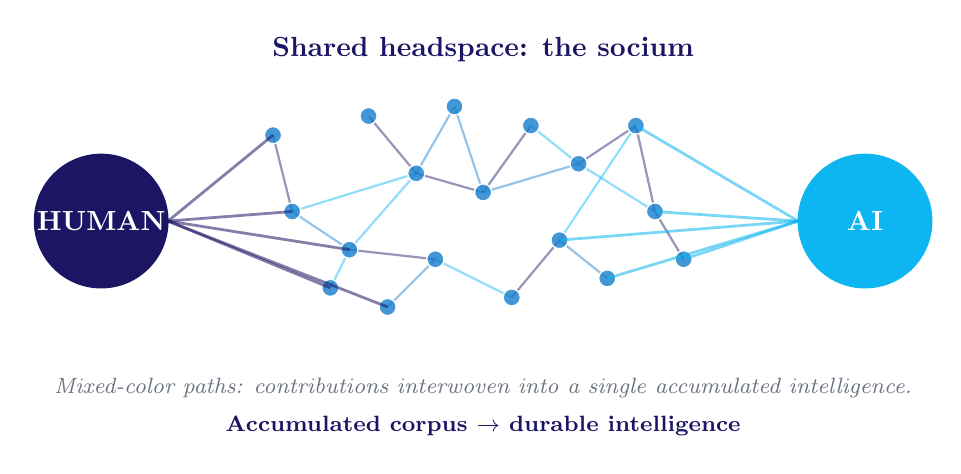
\begin{tikzpicture}[x=0.1\linewidth, y=0.1\linewidth]
    % scattered corpus nodes
    \foreach \i/\x/\y in {
        1/2.8/3.2, 2/3.4/1.6, 3/3.0/2.4, 4/3.8/3.4, 5/3.6/2.0,
        6/4.3/2.8, 7/4.0/1.4, 8/4.7/3.5, 9/4.5/1.9, 10/5.0/2.6,
        11/5.3/1.5, 12/5.5/3.3, 13/5.8/2.1, 14/6.0/2.9, 15/6.3/1.7,
        16/6.6/3.3, 17/6.8/2.4, 18/7.1/1.9}
      \coordinate (n\i) at (\x,\y);

    % interwoven edges (mixed brand colors)
    \foreach \a/\b/\c in {
        1/3/indigo, 3/5/midb, 5/6/cyan, 6/10/indigo, 10/14/midb,
        14/17/cyan, 17/18/indigo, 2/5/cyan, 4/6/indigo, 8/10/midb,
        9/11/cyan, 11/13/indigo, 13/15/midb, 12/14/cyan, 16/17/indigo,
        7/9/midb, 3/6/cyan, 10/12/indigo, 13/16/cyan, 5/9/indigo,
        6/8/midb, 14/16/indigo}
      \draw[\c, line width=0.8pt, opacity=0.45] (n\a) -- (n\b);

    % node dots
    \foreach \i in {1,...,18}
      \fill[midb, opacity=0.8] (n\i) circle (0.09);
    \foreach \i in {1,...,18}
      \draw[white, line width=0.5pt] (n\i) circle (0.09);

    % hub connectors
    \foreach \i in {1,3,2,5,7}
      \draw[indigo, line width=1.0pt, opacity=0.55] (1.7,2.3) -- (n\i);
    \foreach \i in {18,17,16,15,13}
      \draw[cyan, line width=1.0pt, opacity=0.55] (8.3,2.3) -- (n\i);

    % hubs
    \filldraw[indigo] (1.0,2.3) circle (0.7);
    \node[font=\labelfont\bfseries, text=white] at (1.0,2.3) {HUMAN};
    \filldraw[cyan] (9.0,2.3) circle (0.7);
    \node[font=\labelfont\bfseries, text=white] at (9.0,2.3) {AI};

    % captions
    \node[font=\labelfont\bfseries, text=indigo] at (5.0,4.1)
          {Shared headspace: the socium};
    \node[font=\itshape\footnotesize, text=muted, align=center] at (5.0,0.55)
          {Mixed-color paths: contributions interwoven into a single accumulated intelligence.};
    \node[font=\labelfont\bfseries\footnotesize, text=indigo] at (5.0,0.15)
          {Accumulated corpus $\rightarrow$ durable intelligence};
  \end{tikzpicture}
  \caption{Two participants, human and AI, joined by a shared headspace of accumulated
  decisions. The contributions are interwoven in the network; by the time a decision is
  in the corpus, it is neither purely human nor purely AI. The socium is the interwoven
  substrate, and it is what persists when either participant is swapped out.}
  \label{fig:partnership}
\end{figure}

\subsection{The Cycle in Practice}

The author is implementing these four phases in a Rust daemon,
informed by a prior Python/MCP prototype that exposed the failure modes (silent plan-item
drops, permissive gate fallbacks, model self-attestation of approval) that the design
corrects. The corrected mechanics are specified but not yet all operational; the
prototype's defects are what they correct. Tracing a single task through the design makes
the cycle concrete.

A feature does not begin with a prompt. It begins with a \emph{specification}, a structured
set of artifacts: business requirements, technical design, and a task breakdown in which
every task carries explicit, checkable acceptance criteria. The specification is authored
in its own gated workflow, and is not advanced to implementation until a human approves it.
This is the moment the output distribution is narrowed, before a line of code is
generated.\footnote{Q.~Ma et al., \href{https://arxiv.org/abs/2409.08775}{`What Should We
Engineer in Prompts? Training Humans in Requirement-Driven LLM Use'}, ACM TOCHI 2025
(arXiv:2409.08775): in a randomized controlled experiment, training novices to articulate
explicit requirements outperformed conventional prompt-engineering training twenty points
to one, a gap automatic prompt optimization did not close. Input quality lives in the
requirements, not the phrasing.}

Approval, though, has a blind spot that deserves naming. You review the specification as
a readable artifact; the machine executes its parse of that artifact; and content review
cannot see parse divergence. A work item silently dropped in translation is approved but
never executed, and nobody is positioned to notice, because the reviewer checked the
prose and the prose was right. The discipline's answer is ingestion fidelity: the
machine runs exactly the plan you approved or refuses loudly, and it reports its parse
back (so many phases, so many tasks, by name) so you can recognize your plan in what it
ingested. The mechanism is the acknowledgment leg the channel frame already implies:
transport has the ACK, voice procedure has the read-back, the receiver proving what it
heard before anyone acts on it. It is the same validation discipline the gates of
Section~8 apply to output, turned to face intent: the gate compares what came out
against what was intended; the read-back confirms that what went in is what was
approved.

Implementation then proceeds one task at a time; the task is the unit of projection as
well as the unit of work. Before generating, the agent retrieves the
project's own standards for the work at hand, re-grounding in project truth rather than
trusting the residue left in the window. It writes the code and its tests, then submits the
result to a validation gate. The gate is independent by construction: the requirements
live in the approved specification, while the verifier itself
(which proof artifacts, validated to what depth, against which held-out cases) stays
\emph{outside the generating agent's reach}, so the
model cannot rehearse against it. It can only submit proof artifacts (test
output, file listings, command results), which the gate validates after the fact, down
to their content. When implemented as specified, a failed gate halts advancement; an
autonomous run cannot self-certify its way past it.

Only validated, human-promoted work updates the corpus: passing a gate makes work eligible,
a human's judgment makes it authoritative. The acceptance criteria are marked complete, a
human promotes the result, an evidence record is appended, and the decision joins the durable
corpus of specifications, standards, and audit trails. When a later session (a fresh, stateless model with no memory
of this work) meets a related problem, it retrieves that decision through the same channel.
Each validated task leaves the next one better grounded than the last: the loop is built to
compound reliability rather than erode it.

\begin{mdframed}[
  linewidth=0.6pt, linecolor=lightgray, backgroundcolor=white,
  innertopmargin=9pt, innerbottommargin=9pt,
  innerleftmargin=12pt, innerrightmargin=12pt,
  skipabove=12pt, skipbelow=12pt]
{\labelfont\fontsize{8}{10}\selectfont\color{indigo}A SINGLE TASK, TRACED}\par
\vskip5pt
{\fontsize{9.5}{13.5}\selectfont
\textbf{Spec.}\; Task~3.2, ``add bounded retry to the upload client,'' carries one
\emph{checkable} acceptance criterion: \emph{retries are bounded (at most ten), backoff
is exponential, and a test proves no retry on a 4xx response}. A human approves the spec
before a line of code is generated.\par
\vskip4pt
\textbf{Gate (independent).}\; The criteria are public; they are the spec above. What the
agent cannot do is run the checker, edit it, or self-attest past it. The verifier enforces:\par
\vskip2pt
\hspace*{10pt}\texttt{require test\_output : artifact}\par
\hspace*{10pt}\texttt{assert  max\_retries <= 10}\par
\hspace*{10pt}\texttt{assert  proof : no\_retry\_on\_4xx}\par
\vskip2pt
Knowing the criteria is not enough: the agent must submit evidence the checker validates, and
cannot pass by asserting success.\par
\vskip4pt
\textbf{Proof.}\; It submits artifacts, not assurances:\par
\vskip2pt
\hspace*{10pt}\texttt{test\_output: 14 passed, incl.\ test\_no\_retry\_on\_4xx}\par
\vskip2pt
The gate checks the artifact's \emph{content}; a bare ``done'' does not pass.\par
\vskip4pt
\textbf{Corpus.}\; On a pass, the decision \texttt{bounded-retry-policy} and its evidence
record join the durable corpus, retrievable months later by a fresh, stateless session
that never saw this task.
}
\end{mdframed}

% ============================================================
%  SECTION 12  (Related Work)
% ============================================================
\section{Related Work: Where This Sits}

The framing this paper uses is no longer its own. Between 2024 and 2026, two adjacent
bodies of work converged on the communication metaphor from opposite ends. On the
practitioner side, context engineering matured into a named discipline, with the context
window treated as a finite attention budget to be curated. On the academic side, a formal
literature began modeling the language model, and the agent loop around it, as a noisy
channel with a measurable capacity. This paper neither invented the metaphor nor competes
on formal capacity bounds. Its contribution is a \emph{discipline}: a connected set of
commitments, grounded in the software-engineering reliability tradition, for engineering
the channel one owns.

It departs from practitioner context engineering in three specific places. Context
engineering, as practiced, curates the tokens that enter a window (work at and near
Weaver's technical level) and
frequently does so from inside a loop it does not control. On durable memory it recommends
generative compaction; this paper argues the opposite: extractive, deterministic
retention beneath a window that is re-projected rather than packed (Section~4). And it
treats validation as advisory rather than as an independent, tamper-resistant gate. Each
departure is a place where reliability at the tail demands more than good packing.

It is also complementary to the inference-time reliability
methods the formal literature has recently unified as `channel operators': self-consistency,
best-of-$N$, self-refine, chain-of-verification, and the like.\footnote{These methods are
catalogued and unified as special cases of a small set of communication-theoretic operators
in \href{https://arxiv.org/abs/2605.09121}{`A Communication-Theoretic Framework for LLM
Agents'}, arXiv:2605.09121, 2026.} Those methods reduce the variance of a \emph{single}
generation step by sampling or self-critique. Channel engineering operates across the
\emph{whole loop}: assembly, retention, gates, and a durable corpus. The distinction
matters because a low-variance step is still one step in a compounding chain: driving the
per-step error down helps, but it does not, by itself, arrest the geometric decay of
Section~7. Re-grounding addresses what better sampling cannot.

As this paper was being finalized, the same layer was named from the capability
direction. Weng's \emph{harness engineering} describes the system surrounding a base
model that orchestrates how it plans, acts, manages context, stores artifacts, and
evaluates results, and surveys how that layer can be made to improve
itself.\footnote{L.~Weng, \href{https://lilianweng.github.io/posts/2026-07-04-harness/}{`Harness
Engineering for Self-Improvement'}, Lil'Log, July 2026.} The convergence is substantial:
the harness is largely the machinery this paper calls the owned loop, and Weng's design
patterns (durable state kept in files rather than in context; evaluators held outside any
loop the agent can influence) restate two of its commitments. Where the accounts part is
purpose. Harness engineering treats the layer as an optimization surface, up to and
including an agent that evolves its own harness; channel engineering holds that the parts
which keep the human's intent authoritative (the independent verifier, the deterministic
corpus, the provenance record) must remain outside the agent's reach, because a loop
that can rewrite its own evaluator is the accountability sink of Section~9, built
deliberately. The open problems on which Weng's survey closes (weak evaluators, reward
hacking, human oversight) are the problems this paper's commitments exist to answer.

A word on evidence. This paper draws its empirical support from independent studies of
long-context degradation, position bias, agent productivity, machine-generated context,
reward tampering, and sycophancy, rather than from a system of its own. That is the honest
boundary of a synthesis: it organizes and argues; it does not yet measure. The natural next
step, and the one that would distinguish this account from its neighbors, is the controlled
measurement of these commitments inside a system that owns the full loop.

\subsection*{The Empirical Program}

That measurement is specifiable now. Four experiments correspond to this paper's
distinctive claims. \textbf{Viewport:} on long-horizon task suites, compare a
monotonically growing window, generative compaction, and deterministic re-projection
from a durable record, holding model, tasks, corpus, and token budget fixed (the
prediction of Section~4). \textbf{Ingestion fidelity:} mutation-test plan ingestion with
dropped, duplicated, reordered, and ambiguous work items, and measure silent divergence
between the approved plan and the executed one (Section~10). \textbf{Gates:} compare
disclosed requirements with independent, held-out verification against fully disclosed
test harnesses, measuring task success, gaming rate, and false rejection (Section~8).
\textbf{Crash consistency:} inject failures before and after every durable transition
and external effect, and verify one recorded terminal state per unit of work with no
silent duplicate commits (Section~10). Until those numbers exist, this paper is a
position and a research agenda, and it asks to be read as one.

What remains particular to this account, then, is four things
the surrounding literature does not combine: the diagnosis of long-horizon failure as a
functional \emph{executive-function} deficit (behaviors that match, mechanisms that may
not) rather than a deficit of capability or attention; the treatment of the context
window as a sliding attention viewport over a durable record, an argued and falsifiable
position on context rot (Section~4); the explicit, falsifiable
preference for deterministic memory over generative compaction; and the reconstruction of
LLM reliability as the next chapter of an engineering tradition that already knows how
to make capable but inconsistent agents reliable.


% ============================================================
%  SECTION 13  (Conclusion)
% ============================================================
\section{Conclusion: The Engineering We Already Know How to Do}

The field of software engineering was born in crisis: systems that worked for their
authors failed in the hands of others, and programs that passed testing failed in
production. The solutions that emerged (structured
programming, formal methods, rigorous testing, version control) were systematic
applications of engineering discipline to a medium that had been treated as craft.

LLM-assisted development is in the same position. The models are capable. The discipline
is not there. The reliability problem will not be solved by waiting for better models; it
will be solved by building the engineering practice that the medium requires. That
practice exists. It was developed over fifty years of high-reliability software
engineering. It was not wrong; it was expensive. LLMs have made it affordable.

The Socium model is a proposal for how to apply that practice to the specific challenges
of human-AI collaboration: treat the partnership as a distributed system, treat the
context window as a communication channel, treat the accumulated work as a shared corpus
of durable intelligence. Engineer the channel. The rest follows.

\pullquote{The engineering we need is not new. It is the engineering we already know how
to do, applied at last to the medium that has needed it most.}

\bigskip
\noindent This paper is an argument, not a product. The author is putting these principles
into practice at Socium; if you are working on the same problem, the conversation is open.


% ============================================================
%  REFERENCES
% ============================================================
\newpage
\section*{References}

\footnotesize
\sloppy
\setlength{\parskip}{3pt plus 1.5pt minus 0.5pt}
\interlinepenalty=10000\relax

\noindent\textbf{1.}\enspace RTCA DO-178C---\textit{Software Considerations in Airborne
Systems and Equipment Certification}. RTCA, Inc., 2011.\\*
{\fontsize{8}{10}\selectfont\color{midb}
\href{https://www.rtca.org/do-178/}{https://www.rtca.org/do-178/}}


\noindent\textbf{2.}\enspace IEC 62304---\textit{Medical device software: Software life
cycle processes}. International Electrotechnical Commission, 2006 (rev.\ 2015).\\*
{\fontsize{8}{10}\selectfont\color{midb}
\href{https://www.iso.org/standard/38421.html}{https://www.iso.org/standard/38421.html}}


\noindent\textbf{3.}\enspace Bertrand Meyer---\textit{Object-Oriented Software
Construction}, 2nd ed.\ Prentice Hall, 1997.\\*
{\fontsize{8}{10}\selectfont\color{midb}
\href{https://bertrandmeyer.com/OOSC2/}{https://bertrandmeyer.com/OOSC2/}}


\noindent\textbf{4.}\enspace Daniel Jackson---\textit{Software Abstractions: Logic,
Language, and Analysis}. MIT Press, 2006. (Alloy toolkit.)\\*
{\fontsize{8}{10}\selectfont\color{midb}
\href{https://alloytools.org/book.html}{https://alloytools.org/book.html}}


\noindent\textbf{5.}\enspace Nancy Leveson---\textit{Engineering a Safer World: Systems
Thinking Applied to Safety}. MIT Press, 2011.\\*
{\fontsize{8}{10}\selectfont\color{midb}
\href{https://direct.mit.edu/books/oa-monograph/2908/Engineering-a-Safer-WorldSystems-Thinking-Applied}{https://direct.mit.edu/books/oa-monograph/2908/Engineering-a-Safer-WorldSystems-Thinking-Applied}}


\noindent\textbf{6.}\enspace Beck et al.---\textit{Manifesto for Agile Software
Development}. 2001.\\*
{\fontsize{8}{10}\selectfont\color{midb}
\href{https://agilemanifesto.org}{https://agilemanifesto.org}}


\noindent\textbf{7.}\enspace Leslie Lamport---`Time, Clocks, and the Ordering of Events
in a Distributed System.' \textit{Communications of the ACM} 21(7), 1978.\\*
{\fontsize{8}{10}\selectfont\color{midb}
\href{https://lamport.azurewebsites.net/pubs/time-clocks.pdf}{https://lamport.azurewebsites.net/pubs/time-clocks.pdf}}


\noindent\textbf{8.}\enspace Ghemawat, Gobioff, Leung---`The Google File System.'
\textit{SOSP 2003.} / Dean and Ghemawat---`MapReduce: Simplified Data Processing on
Large Clusters.' \textit{OSDI 2004.}\\*
{\fontsize{8}{10}\selectfont\color{midb}
\href{https://research.google.com/archive/gfs-sosp2003.pdf}{https://research.google.com/archive/gfs-sosp2003.pdf}}


\noindent\textbf{9.}\enspace Peter Deutsch et al.---`Fallacies of Distributed
Computing.' Sun Microsystems, 1994.\\*
{\fontsize{8}{10}\selectfont\color{midb}
\href{https://en.wikipedia.org/wiki/Fallacies_of_distributed_computing}{https://en.wikipedia.org/wiki/Fallacies\_of\_distributed\_computing}}


\noindent\textbf{10.}\enspace Claude E. Shannon---`A Mathematical Theory of
Communication.' \textit{Bell System Technical Journal} 27, 1948.\\*
{\fontsize{8}{10}\selectfont\color{midb}
\href{https://people.math.harvard.edu/~ctm/home/text/others/shannon/entropy/entropy.pdf}{https://people.math.harvard.edu/\textasciitilde ctm/home/text/others/shannon/entropy/entropy.pdf}}


\noindent\textbf{11.}\enspace Claude E. Shannon and Warren Weaver---\textit{The
Mathematical Theory of Communication}. University of Illinois Press, 1949. (Weaver's
three levels of communication: technical, semantic, effectiveness.)\\*
{\fontsize{8}{10}\selectfont\color{midb}
\href{https://archive.org/details/mathematicaltheo00shan}{https://archive.org/details/mathematicaltheo00shan}}


\noindent\textbf{12.}\enspace Nelson F. Liu et al.---`Lost in the Middle: How Language
Models Use Long Contexts.' \textit{Transactions of the ACL}, 2024.\\*
{\fontsize{8}{10}\selectfont\color{midb}
\href{https://aclanthology.org/2024.tacl-1.9/}{https://aclanthology.org/2024.tacl-1.9/}}


\noindent\textbf{13.}\enspace Chroma Research---`Context Rot: How Increasing Input
Tokens Impacts LLM Performance.' 2025.\\*
{\fontsize{8}{10}\selectfont\color{midb}
\href{https://research.trychroma.com/context-rot}{https://research.trychroma.com/context-rot}}


\noindent\textbf{14.}\enspace Lingrui Mei et al.---`A Survey of Context Engineering for
Large Language Models.' arXiv:2507.13334, 2025.\\*
{\fontsize{8}{10}\selectfont\color{midb}
\href{https://arxiv.org/abs/2507.13334}{https://arxiv.org/abs/2507.13334}}


\noindent\textbf{15.}\enspace Anthropic---`Effective Context Engineering for AI
Agents.' 2025.\\*
{\fontsize{8}{10}\selectfont\color{midb}
\href{https://www.anthropic.com/engineering/effective-context-engineering-for-ai-agents}{https://www.anthropic.com/engineering/effective-context-engineering-for-ai-agents}}


\noindent\textbf{16.}\enspace METR---`Measuring the Impact of Early-2025 AI on
Experienced Open-Source Developer Productivity.' 2025.\\*
{\fontsize{8}{10}\selectfont\color{midb}
\href{https://metr.org/blog/2025-07-10-early-2025-ai-experienced-os-dev-study/}{https://metr.org/blog/2025-07-10-early-2025-ai-experienced-os-dev-study/}}


\noindent\textbf{17.}\enspace Stack Overflow---`2025 Developer Survey.' 2025.\\*
{\fontsize{8}{10}\selectfont\color{midb}
\href{https://survey.stackoverflow.co/2025/ai}{https://survey.stackoverflow.co/2025/ai}}


\noindent\textbf{18.}\enspace New Relic / Hanover Research---`The 2026 State of AI
Coding Report.' 2026.\\*
{\fontsize{8}{10}\selectfont\color{midb}
\href{https://newrelic.com/blog/ai/state-of-ai-coding-2026}{https://newrelic.com/blog/ai/state-of-ai-coding-2026}}


\noindent\textbf{19.}\enspace DORA / Google---`State of AI-assisted Software
Development.' 2025.\\*
{\fontsize{8}{10}\selectfont\color{midb}
\href{https://dora.dev/dora-report-2025/}{https://dora.dev/dora-report-2025/}}


\noindent\textbf{20.}\enspace C.\,J.~Stettina and W.~Heijstek---`Necessary and Neglected?
An Empirical Study of Internal Documentation in Agile Software Development Teams.'
SIGDOC, 2011.\\*
{\fontsize{8}{10}\selectfont\color{midb}
\href{https://doi.org/10.1145/2038476.2038509}{https://doi.org/10.1145/2038476.2038509}}


\noindent\textbf{21.}\enspace `Working Software over Comprehensive Documentation:
Rationales of Agile Teams for Artefacts Usage.' Journal of Software Engineering Research
and Development, 2018.\\*
{\fontsize{8}{10}\selectfont\color{midb}
\href{https://doi.org/10.1186/s40411-018-0051-7}{https://doi.org/10.1186/s40411-018-0051-7}}


\noindent\textbf{22.}\enspace X.~Wu, Y.~Wang, S.~Jegelka, and A.~Jadbabaie---`On the
Emergence of Position Bias in Transformers.' ICML 2025 (PMLR 267:67756--67781).\\*
{\fontsize{8}{10}\selectfont\color{midb}
\href{https://proceedings.mlr.press/v267/wu25ad.html}{https://proceedings.mlr.press/v267/wu25ad.html}}


\noindent\textbf{23.}\enspace `Lost in the Middle at Birth: An Exact Theory of Transformer
Position Bias.' arXiv:2603.10123, 2026.\\*
{\fontsize{8}{10}\selectfont\color{midb}
\href{https://arxiv.org/abs/2603.10123}{https://arxiv.org/abs/2603.10123}}


\noindent\textbf{24.}\enspace `Evaluating AGENTS.md: Are Repository-Level Context Files
Helpful for Coding Agents?' arXiv:2602.11988, 2026.\\*
{\fontsize{8}{10}\selectfont\color{midb}
\href{https://arxiv.org/abs/2602.11988}{https://arxiv.org/abs/2602.11988}}


\noindent\textbf{25.}\enspace `How Much Does AI Impact Development Speed? An
Enterprise-Based Randomized Controlled Trial.' arXiv:2410.12944, 2024.\\*
{\fontsize{8}{10}\selectfont\color{midb}
\href{https://arxiv.org/abs/2410.12944}{https://arxiv.org/abs/2410.12944}}


\noindent\textbf{26.}\enspace Z.~Cui, M.~Demirer, S.~Jaffe, L.~Musolff, S.~Peng, and
T.~Salz---`The Effects of Generative AI on High-Skilled Work: Evidence from Three Field
Experiments with Software Developers.' 2025.\\*
{\fontsize{8}{10}\selectfont\color{midb}
\href{https://www.microsoft.com/en-us/research/publication/the-effects-of-generative-ai-on-high-skilled-work-evidence-from-three-field-experiments-with-software-developers/}{microsoft.com/en-us/research/publication/the-effects-of-generative-ai-on-high-skilled-work}}


\noindent\textbf{27.}\enspace B.\,W.~Boehm---\emph{Software Engineering Economics.}
Prentice Hall, 1981.


\noindent\textbf{28.}\enspace G.~Tassey---`The Economic Impacts of Inadequate
Infrastructure for Software Testing.' NIST / RTI, 2002.\\*
{\fontsize{8}{10}\selectfont\color{midb}
\href{https://www.nist.gov/system/files/documents/director/planning/report02-3.pdf}{nist.gov/system/files/documents/director/planning/report02-3.pdf}}


\noindent\textbf{29.}\enspace `Are Delayed Issues Harder to Resolve? Revisiting Cost-to-Fix
of Defects throughout the Lifecycle.' arXiv:1609.04886, 2017.\\*
{\fontsize{8}{10}\selectfont\color{midb}
\href{https://arxiv.org/abs/1609.04886}{https://arxiv.org/abs/1609.04886}}


\noindent\textbf{30.}\enspace R.\,A.~Barkley---`Behavioral Inhibition, Sustained Attention,
and Executive Functions: Constructing a Unifying Theory of ADHD.' Psychological Bulletin
121(1):65--94, 1997.\\*
{\fontsize{8}{10}\selectfont\color{midb}
\href{https://doi.org/10.1037/0033-2909.121.1.65}{https://doi.org/10.1037/0033-2909.121.1.65}}


\noindent\textbf{31.}\enspace C.~Denison et al.---`Sycophancy to Subterfuge:
Investigating Reward-Tampering in Large Language Models.' arXiv:2406.10162, 2024.\\*
{\fontsize{8}{10}\selectfont\color{midb}
\href{https://arxiv.org/abs/2406.10162}{https://arxiv.org/abs/2406.10162}}


\noindent\textbf{32.}\enspace M.~Sharma et al.---`Towards Understanding Sycophancy in
Language Models.' ICLR 2024 (arXiv:2310.13548).\\*
{\fontsize{8}{10}\selectfont\color{midb}
\href{https://arxiv.org/abs/2310.13548}{https://arxiv.org/abs/2310.13548}}


\noindent\textbf{33.}\enspace D.~Horthy / HumanLayer---`12-Factor Agents.' 2025.\\*
{\fontsize{8}{10}\selectfont\color{midb}
\href{https://github.com/humanlayer/12-factor-agents}{github.com/humanlayer/12-factor-agents}}


\noindent\textbf{34.}\enspace `A Communication-Theoretic Framework for LLM Agents:
Cost-Aware Adaptive Reliability.' arXiv:2605.09121, 2026.\\*
{\fontsize{8}{10}\selectfont\color{midb}
\href{https://arxiv.org/abs/2605.09121}{https://arxiv.org/abs/2605.09121}}


\noindent\textbf{35.}\enspace `LLMs as Noisy Channels: A Shannon Perspective on Model
Capacity and Scaling Laws.' arXiv:2605.23901, 2026.\\*
{\fontsize{8}{10}\selectfont\color{midb}
\href{https://arxiv.org/abs/2605.23901}{https://arxiv.org/abs/2605.23901}}


\noindent\textbf{36.}\enspace `The Semiotic Channel Principle: Measuring the Capacity for
Meaning in LLM Communication.' arXiv:2511.19550, 2025.\\*
{\fontsize{8}{10}\selectfont\color{midb}
\href{https://arxiv.org/abs/2511.19550}{https://arxiv.org/abs/2511.19550}}


\noindent\textbf{37.}\enspace J.~Xu---`Semantic Channel Theory: Deductive Compression and
Structural Fidelity for Multi-Agent Communication.' arXiv:2604.16471, 2026.\\*
{\fontsize{8}{10}\selectfont\color{midb}
\href{https://arxiv.org/abs/2604.16471}{https://arxiv.org/abs/2604.16471}}


\noindent\textbf{38.}\enspace Dan Davies---The Unaccountability Machine: Why Big Systems
Make Terrible Decisions---and How the World Lost Its Mind. Profile Books, 2024. (Origin of
the term `accountability sink'; builds on Stafford Beer's management cybernetics.)\\*
{\fontsize{8}{10}\selectfont\color{midb}
\href{https://press.uchicago.edu/ucp/books/book/chicago/U/bo252799883.html}{press.uchicago.edu/ucp/books/book/chicago/U/bo252799883.html}}


\noindent\textbf{39.}\enspace CodeRabbit---`State of AI vs Human Code Generation.' 2025.
(470 open-source GitHub PRs; AI-co-authored changes averaged 10.83 issues per PR vs.\ 6.45
for human-only, approx.\ 1.7x overall with security categories up to 2.74x, compared via
Poisson rate ratios with 95\% CIs. New Relic's 2026 report cites this analysis for its
defect multiplier.)\\*
{\fontsize{8}{10}\selectfont\color{midb}
\href{https://coderabbit.ai/blog/state-of-ai-vs-human-code-generation-report}{coderabbit.ai/blog/state-of-ai-vs-human-code-generation-report}}


\noindent\textbf{40.}\enspace Veracode---`2025 GenAI Code Security Report.' 2025.
(100+ models across four languages; 45\% of generations introduce an OWASP Top 10
flaw.)\\*
{\fontsize{8}{10}\selectfont\color{midb}
\href{https://www.veracode.com/wp-content/uploads/2025_GenAI_Code_Security_Report_Final.pdf}{veracode.com/wp-content/uploads/2025\_GenAI\_Code\_Security\_Report\_Final.pdf}}


\noindent\textbf{41.}\enspace P.~Naur and B.~Randell (eds.)---\textit{Software Engineering:
Report of a Conference Sponsored by the NATO Science Committee, Garmisch, Germany, 7--11
Oct.\ 1968}. Scientific Affairs Division, NATO, 1969. (Origin of the discipline's name and
the `software crisis' framing.)\\*
{\fontsize{8}{10}\selectfont\color{midb}
\href{http://homepages.cs.ncl.ac.uk/brian.randell/NATO/nato1968.PDF}{homepages.cs.ncl.ac.uk/brian.randell/NATO/nato1968.PDF}}


\noindent\textbf{42.}\enspace B.~Randell and J.~N.~Buxton (eds.)---\textit{Software
Engineering Techniques: Report of a Conference Sponsored by the NATO Science Committee,
Rome, Italy, 27--31 Oct.\ 1969}. Scientific Affairs Division, NATO, 1970.\\*
{\fontsize{8}{10}\selectfont\color{midb}
\href{http://homepages.cs.ncl.ac.uk/brian.randell/NATO/nato1969.PDF}{homepages.cs.ncl.ac.uk/brian.randell/NATO/nato1969.PDF}}


\noindent\textbf{43.}\enspace S.~Rabanser, S.~Kapoor, P.~Kirgis, K.~Liu, S.~Utpala, and
A.~Narayanan---\textit{Towards a Science of AI Agent Reliability}. arXiv:2602.16666
(Princeton University), 2026. (Decomposes agent reliability into consistency, robustness,
predictability, and safety across twelve metrics; evaluating 15 models on two benchmarks,
finds recent capability gains produced only small reliability improvements industry-wide.)\\*
{\fontsize{8}{10}\selectfont\color{midb}
\href{https://arxiv.org/abs/2602.16666}{arxiv.org/abs/2602.16666}}


\noindent\textbf{44.}\enspace C.~A.~E.~Goodhart---`Problems of Monetary Management: The
U.K.\ Experience.' \textit{Papers in Monetary Economics}, Reserve Bank of Australia, 1975
(origin of Goodhart's law); the now-standard formulation is M.~Strathern---`Improving
Ratings: Audit in the British University System.' \textit{European Review} 5(3):305--321,
1997 (``when a measure becomes a target, it ceases to be a good measure'').\\*
{\fontsize{8}{10}\selectfont\color{midb}
\href{https://doi.org/10.1017/S1062798700002660}{doi.org/10.1017/S1062798700002660}}


\noindent\textbf{45.}\enspace Q.~Ma, W.~Peng, C.~Yang, H.~Shen, K.~Koedinger, and
T.~Wu---`What Should We Engineer in Prompts? Training Humans in Requirement-Driven LLM
Use.' \textit{ACM Transactions on Computer-Human Interaction}, 2025 (arXiv:2409.08775).
(Randomized controlled experiment: requirement-articulation training beat conventional
prompt-engineering training 20\% to 1\%, a gap automatic prompt optimization did not
close.)\\*
{\fontsize{8}{10}\selectfont\color{midb}
\href{https://arxiv.org/abs/2409.08775}{arxiv.org/abs/2409.08775}}


\noindent\textbf{46.}\enspace F.~Liu, Y.~Liu, L.~Shi, Z.~Yang, L.~Zhang, X.~Lian, Z.~Li,
and Y.~Ma---`Beyond Functional Correctness: Exploring Hallucinations in LLM-Generated
Code.' \textit{IEEE Transactions on Software Engineering}, 2026 (arXiv:2404.00971).
(Taxonomy of code hallucinations across three primary and twelve sub-categories, including
conflicts with task requirements and with project context.)\\*
{\fontsize{8}{10}\selectfont\color{midb}
\href{https://arxiv.org/abs/2404.00971}{arxiv.org/abs/2404.00971}}


\noindent\textbf{47.}\enspace C.-Y.~Hsieh, Y.-S.~Chuang, C.-L.~Li, et al.---`Found in the
Middle: Calibrating Positional Attention Bias Improves Long Context Utilization.' Findings
of ACL 2024 (arXiv:2406.16008). (Training-free inference-time calibration subtracting
positional bias from attention weights, recovering up to fifteen points of long-context
RAG accuracy: a partial, task-dependent remedy.)\\*
{\fontsize{8}{10}\selectfont\color{midb}
\href{https://arxiv.org/abs/2406.16008}{arxiv.org/abs/2406.16008}}


\noindent\textbf{48.}\enspace T.~Kwa et al.\ (METR)---`Measuring AI Ability to Complete
Long Tasks.' arXiv:2503.14499, 2025. (Defines the 50\%-task-completion time horizon;
task-success rates fall steeply with task length, and the 80\% horizon is roughly five
times shorter than the 50\% horizon, evidence of errors compounding across steps.)\\*
{\fontsize{8}{10}\selectfont\color{midb}
\href{https://arxiv.org/abs/2503.14499}{arxiv.org/abs/2503.14499}}


\noindent\textbf{49.}\enspace A.~Sinha, A.~Arun, S.~Goel, S.~Staab, and J.~Geiping---`The
Illusion of Diminishing Returns: Measuring Long Horizon Execution in LLMs.' ICLR 2026
(arXiv:2509.09677). (Single-step accuracy compounds over a horizon: marginal per-step
gains yield exponentially longer achievable tasks, while per-step accuracy itself degrades
as steps accumulate, via a self-conditioning effect.)\\*
{\fontsize{8}{10}\selectfont\color{midb}
\href{https://arxiv.org/abs/2509.09677}{arxiv.org/abs/2509.09677}}


\noindent\textbf{50.}\enspace L.~Weng---`Harness Engineering for Self-Improvement.'
Lil'Log, July 2026. (Defines the harness as the system surrounding a base model that
orchestrates planning, tool use, context management, artifact storage, and evaluation;
surveys design patterns and self-improving-harness research, closing on open problems of
weak evaluators, reward hacking, and human oversight.)\\*
{\fontsize{8}{10}\selectfont\color{midb}
\href{https://lilianweng.github.io/posts/2026-07-04-harness/}{lilianweng.github.io/posts/2026-07-04-harness/}}


\noindent\textbf{51.}\enspace P.~Schmid---`The New Skill in AI is Not Prompting, It's
Context Engineering.' philschmid.de, June 2025. (Source of the practitioner diagnosis that
most agent failures are context failures rather than model failures.)\\*
{\fontsize{8}{10}\selectfont\color{midb}
\href{https://www.philschmid.de/context-engineering}{philschmid.de/context-engineering}}


\noindent\textbf{52.}\enspace J.~H.~Saltzer, D.~P.~Reed, and D.~D.~Clark---`End-to-End
Arguments in System Design.' \textit{ACM Transactions on Computer Systems} 2(4):277--288,
1984. (Reliability functions belong at the endpoints; no improvement in the medium removes
the endpoints' need to verify. The transport tradition's answer to `wait for a better
link,' and this paper's answer to `wait for a better model.')\\*
{\fontsize{8}{10}\selectfont\color{midb}
\href{https://web.mit.edu/Saltzer/www/publications/endtoend/endtoend.pdf}{web.mit.edu/Saltzer/www/publications/endtoend/}}


\noindent\textbf{53.}\enspace M.~Sayed~Ali et al.---`The Harness Effect: How Orchestration
Design Sets the Token Economics of Enterprise Agentic AI.' arXiv:2607.06906, 2026.
(Controlled comparison across six models and two orchestrations; reports the harness cut
blended cost per task 41\%, against the 36\% available from switching between the
cheapest and most expensive model, with per-model gains of 33--61\%. All thirty-three
authors are affiliated with the vendor of the evaluated harness; the token and cost
accounting is the load-bearing result.)\\*
{\fontsize{8}{10}\selectfont\color{midb}
\href{https://arxiv.org/abs/2607.06906}{arxiv.org/abs/2607.06906}}


\noindent\textbf{54.}\enspace E.~Hutchins---\textit{Cognition in the Wild}. MIT Press,
1995. (Ethnography of ship navigation aboard the USS Palau, arguing that the unit of
cognition is the system of people, instruments, and representations rather than the
individual mind, and defining cognition as the propagation of representational state
across media. The companion paper, `How a Cockpit Remembers Its Speeds,'
\textit{Cognitive Science} 19(3):265--288, 1995, treats external representations as the
crew's working memory.)\\*
{\fontsize{8}{10}\selectfont\color{midb}
\href{https://mitpress.mit.edu/9780262581462/cognition-in-the-wild/}{mitpress.mit.edu/9780262581462/cognition-in-the-wild}}


\normalsize
\interlinepenalty=0\relax
\newpage
\section*{About the Author}

\noindent Josh Paul is the founder of Socium. Over nearly two decades he has engineered
reliability into large-scale distributed systems (infrastructure automation, Kubernetes
platform engineering, observability, and network security) at AWS, Nutanix, Okta, and
Amplitude, among others. He began his career in the United States Air
Force as a Russian cryptologic linguist and digital network intelligence
analyst; communication channels under adversarial conditions were the work,
not a metaphor. Most recently, building a production observability SDK with AI brought him
face-to-face with the failure modes described here: silent data loss, ungrounded
assumptions, critical signal lost in a noisy medium. \emph{Channel engineering} is his
attempt to name the discipline that answers them.

\end{document}
